% -------------------------------
% == REPORT 3 ==
% -------------------------------
% -------------------------------
% Madison: Odd numbered sections
% Jake: Even numbered sections
% -------------------------------
% -------------------------------
%

\documentclass[conf]{new-aiaa}

\usepackage[utf8]{inputenc}
\usepackage{float}
\usepackage{graphicx}
\usepackage{amsmath}
\usepackage[version=4]{mhchem}
\usepackage{siunitx}
\usepackage{longtable,tabularx}
\setlength\LTleft{0pt} 
\usepackage{hyperref}
\usepackage{nomencl}
\usepackage{lscape}

\linespread{2}  

\title{Design Report 03: Twin Sea Lion}

\author{
    Madison Junker\footnote{Student ID: 102736535 }, Jacob Killelea\footnote{Student ID: 10550162 } \\
    \emph{ASEN 4138, University of Colorado Boulder, November 16, 2018}
}

\begin{document}

\clearpage
\maketitle
\thispagestyle{empty}

\newpage
\pagenumbering{roman}
\tableofcontents
\addcontentsline{toc}{section}{\listfigurename}
\listoffigures
\addcontentsline{toc}{section}{\listtablename}
\listoftables
\newpage
\printnomenclature[25mm]

\section*{Nomenclature}

{\renewcommand\arraystretch{1.0}
\noindent\begin{longtable*}{@{}l @{\quad=\quad} l@{}}
$AAA$     	               & Advanced Aircraft Analysis Program \\
$AR_W$    	               & Aspect Ratio                       \\
$b_W$	  	               & Wing Span                          \\
$\bar{c}_W$	  	           & Mean Geometric Chord               \\
$i_W$		               & Incidence Angle                    \\
KTAS                       & Knots True Airspeed                \\
$l_f$     	               & Length of fuselage                 \\
$MSL$     	               & Mean Sea Level Altitude            \\
$S_W$     	               & Wing Area                          \\
$TWR$     	               & Thrust to weight ratio             \\
$\epsilon_W$               & Wing Twist Angle                   \\
$\Lambda_{c/4w}$[$^\circ$] & Wing Sweep Angle                   \\
$\lambda_W$	               & Taper Ratio                        \\
$\lambda_{c/4w}$           & Quarter-chord Sweep Angle          \\
$\Gamma_W$	               & Dihedral                           \\
\end{longtable*}}

\newpage
\pagenumbering{arabic}

% 1
\section{Introduction}

\section{Preliminary Weight and Balance Analysis}

\subsection{Preliminary Weight Breakdown}
%Define/show axis system

% Explain the empty weight breakdown of your aircraft, including individual 
\begin{table}
\label{tab:Empty Weight}
\caption{Empty weight breakdown of the Sea Lion.}
\begin{tabular}{|c|c|c|c|c|c|c|}\hline
Fuselage & Wing & Empennage & Landing Gear & Nacelle & Powerplant & Fixed Equipment \\ \hline
4455.5 & 3386.2 & 712.9 & 1639.6 & 855.5 & 5596.2 & 5275.4 \\ \hline
\end{tabular}
\end{table}
% tables with structural, powerplant, and fixed equipment weight breakdowns 
\begin{table}
\label{tab:Structural Weight}
\caption{Structural weight breakdown.}
\begin{tabular}{|c|c|c|c|c|c|}
Wing & Fuselage & Horizontal Tail & Vertical Tail & Nose Gear & Main Gear \\ \hline
3386.2 & 4455.6 & 445.6 & 267.3 & 245.9 & 1399.7 \\ \hline
\end{tabular}
\end{table}

\begin{table}
\label{tab:Powerplant Weight}
\caption{Powerplant weight breakdown.}
\begin{tabular}{|c|c|c|c|}
Engine 1 & Engine 2 & Propeller 1 & Propeller 2 \\ \hline
1896.3 & 1896.3 & 901.8 & 901.8 \\ \hline
\end{tabular}
\end{table}

\begin{table}
\label{tab:Fixed Equipment Weight}
\caption{Fixed equipment $c_g$}
\begin{tabular}{|c|c|}\hline
Lavatory & Other \\ \hline
83.4 & 5192.0 \\ \hline
\end{tabular}
\end{table}
% and the x-,y-, and z-cg locations of the various weight components. You can 
\begin{table}
\label{tab:Structural cg}
\caption{Structural $c_g$ breakdown.}
\begin{tabular}{|c|c|c|c|}
	& $x_{cg}$ [ft] & $y_{cg}$ [ft] & $z_{cg}$ [ft] \\ \hline
Wing & 23 & 0 & 2\\ \hline
Fuselage & 21.41 & 0 & 3.5\\ \hline
Horizontal Tail & 62 & 0 & 6\\ \hline
Vertical Tail & 62	& 0 & 16\\ \hline
Nose Gear & 8 & 0 & 0.98\\ \hline
Main Gear & 30 & 0 & 2.38\\ \hline 
\end{tabular}
\end{table}

\begin{table}
\label{tab:Powerplant cg}
\caption{Powerplant $c_g$ breakdown.}
\begin{tabular}{|c|c|c|c|}\hline
Engine 1 & 23 & 9 & 3\\ \hline
Engine 2 & 23 & -9 & 3\\ \hline
Propeller 1 & 20 & 9 & 3 \\ \hline
Propeller 2 & 20 & -9 & 3\\ \hline
\end{tabular}
\end{table}

\begin{table}
\label{tab:Fixed equipment cg}
\caption{Fixed equipment $c_g$ breakdown.}
\begin{tabular}{|c|c|c|c|}\hline
Lavatory & 41.63 & 1.96 & 4.21\\ \hline
Other & 21.41 & 0 & 3.5\\ \hline

\end{tabular}
\end{table}

% appendix Since the engine weigh 1500 lbs each and our initial weight budget 
% for power plant was 4655.1 lbs, some extra weight for the engines had to be 
% found.
% Explain if you adjusted any weights calculated from the weight fraction 
% table (like the powerplant weight) Give calculations for your lavatory 
% and galley weights, if applicable, and any other detailed weights such as 
% conference tables. Discuss the general method of how you determined component 
% cg locations and how you divided up calculated weights (like tail and gear weights).

From the gerren equation (Pres 18), the propellers have a diameter of 9.25 ft. From AAA, these propellers will weigh about 1800 lbs. With 3000 lbs of engine and about 700 lbs of extra power plant weight (reduced due to electronic actuators).

Power plant weight was determined by dividing the allowed weight in two and subtracting the 901.8 allotted for each side of propeller.

Nose gear was 15\% of the gear weight with the main gear taking the remaining weight. Vertical tail weight was assumed to be 3/8 of allotted tail weight to conform to DHC-6 proportions.

$W_{lav} = 3.9(10^{1.33})=83.38$lbs. Xcg of lavatory is 499.5 inches. Ycg is 23.5 in. Zcg is 50.5 in.

190 inches first guess for wing apex.2 feet for distance from bottom.

Fuselage .45 of length.

7.9 foot long engines suggest about 10 foot long nacelles. This give 4.8 feet behind the 

The tire is 9 inches wide so the z direction offset will be 4.5 inches.

The nose gear tire is 6.5 inches wide

%If you are storing fuel in the fuselage, include a drawing of your fuel tank, including its estimated cg point. Don't forget to include its location in the fuselage for weight and balance calculations

\subsection{Preliminary Weight and Balance Calculation}
%Explain the fully-loaded weight breakdown of your aircraft, including a table with the loaded component weights and x-,y- and z-cg locations. Again, you can "cut and paste" as above.
%Include the loading scenario. Explain how you grouped things (like passengers, munitions, etc.) and determined the order in which items are loaded/unloaded. Show the X-cg and Z-cg excursion plots.
%List the fully-loaded, forward and aft cg locations (need X and Z values for each). Calculated your X-cg shift from most forward to most aft location, and divide by your mean aerodynamic chord. Compare you values (in inches as well as divided by c) with those in Tables 10.3 of Roskam, Part II (posted on Canvas under Technical Documentation).


\section{Empennage Layout Design}
%Present what kind of tail (T-tail, cruciform, or low-mounted) was chosen and why. Also, if any fuel is being stored in the empennage, include a fuel volume calculation

This group selected a conventional tail layout in the interest of simplicity and separation of concerns. The tail and empennage serves only aerodynamic stability and control, so no special features were required.

\subsection{Sizing the Horizontal Stabilizer} %AND/OR canard
%Discuss the location and design of the horizontal stabilizer and/or the canard. Need to include: S, b, AR, Gamma c/4, Lambda, lambda, t/c, and airfoil selected for the horizontal tail and/or canard. Calculate and compare values of Vh and/or Vc to those of similar aircraft
%Include AAA printouts of volume coefficient calculations in the appendix and a drawing of the horizontal stabilizer and/or canard in the chapter itself
%Perform a critical Mach number check for each, if applicable. Mcr plots are found in Canvas. Show where your point lies on the plot

The horizontal stabilizer was designed principally for ensuring that the horizontal tail volume coefficient, $V_h$, lay between 0.7 and 1.1, as seen in \cite{orange_book}, as well as keeping the static margin, fuselage length, and horizontal tail area to reasonable limits. This effort was only a partial success, as a suitable static margin has not yet been found. 

% TODO: what is capital lambda?

The surface area of the horizontal tail is TBD feet. It is TBD feet in span, with a taper ratio, $\lambda$, of TBD. For simplicity, it has no dihedral. The airfoil selected for the tail is a NACA 0012 for its simple construction.

By inspecting figure \ref{fig:critical_mach_check}, the cruise speed of $M-0.6$ is too low for any shock formation. If cruise speed was higher, then a thinner control surface airfoil might be required. However, in this case the thickness of the horizontal stabilizer could safely be increased to just about any reasonable amount without worrying about the formation of shocks.

\subsection{Sizing the Vertical Stabilizer}
%Discuss the location and design of the vertical stabilizer. Need to include: S, b, AR, Gamma c/4, lambda, t/c, and airfoil selected. Calculate and compare values of Vv to those of similar aircraft.
%Include AAA printouts of volume coefficient calculations in the appendix and a drawing of the vertical stabilizer in the chapter itself
%Perform a Mach critical check, if applicable. Again Mcr plots are found in Canvas. Show where your point lies on the plot
%Go to the stability and control module and calculate the static margin, setting eta hp,off =1. This will give you the static margin of your airplane, which is listed as the output parameter, SM. Comment on the results - is your airplane likely to be longitudinally stable? Unstable? If changes need to be made to either the CG (due to weight and balance) and/or the AC (due to wing/tail location), now is the time to make changes.

\section{Control Surface Layout Design}
\subsection{Sizing the Lateral Control Surfaces}
%Include the AAA printout of aileron calculations in the appendix and a drawing of the wing/aileron in the chapter itself
%Include ca/cw, eta ai and eta ao dimensions, and show that the ailerons does not interfere with the flap location. Include spoiler sizing data here if spoilers are needed. Include (Sa/Sw) calculated from your AAA values and compare it with similar aircraft. Comment - based on your valued, do you expect problems with sufficient roll authority?
\subsection{Sizing the Longitudinal Control Surfaces}
%Include AAA printout of elevator and/or canardvator calculations in the appendix and a drawing of the tail/elevator and/or canard/canardvator in the chapter itself
%Include ce/ch, eta eo dimensions (and/or ccv/cc, eta cvi, and eta cvo dimensions). Include (Se/Sh), and/or (Scv/Sc) calcuated from your AAA values and compare them with similar aircraft. Comment - based on your values, do you expect problems with sufficient pitch authority?
%If you have a movable stabilizer with no elevator and/or a movable canard with no canardvator, state and discuss that in this section
\subsection{Sizing the Directional Control Surfaces}
%Include AAA printout of rudder calculations in the appendix and a drawing of the tail/rudder in the chapter itself
%Include cr/cv, eta ti and eta p0 dimensions. Include (Sr/Sv) calculated from your AAA values and compare it with similar aircraft. Comment - based on your values, do you expect problems with sufficient yaw authority?

\section{Landing Gear Layout Design}
\subsection{Sizing of the Landing Gear}
%Describe how you chose the landing gear configuration (tricycle, taildragger, etc) for your aircraft and why.
% Include
	%Fixed or retractable
    %Number of struts ("bogeys")
    %Number of tires per strut and selection of tires (diameter and width)
    %Arrangement of tires (dual, tandem, etc)
    %Maximum static load per bogey (Pn and Pm)
    %Weight distribution % - is it within acceptable bounds?
\subsection{Location of the Landing Gear}
%Describe how you chose the location of the gear for your aircraft
%Show that you meet longitudinal and lateral ground clearance requirements
%Show that you meet longitudinal and lateral tip-over requirements
%Include strut diameters and lengths


\subsection{Gear Retraction Volume}
%If application, discuss your gear retraction volume calculations (with growth factors) for all gear and whether the gear will retract into the wings, into the fuselage, or a bubble fairing on the side of the fuselage. Show your calculations, both for what volume is required for retraction and for what is available in the wing, fuselage, or fairing.

\section{Conclusions and Recommendations}
\subsection{Conclusions}

\subsection{Recommendations}

\begin{thebibliography}{99}

% Todo: orange book charts for Vh and Vv

\bibitem{pres13} Gerren, "Presentation 13", \url{https://canvas.colorado.edu}

\end{thebibliography}

% 8
\section{Appendix}

\subsection{AAA: Preliminary Weight Analysis}
\begin{figure}[H]
    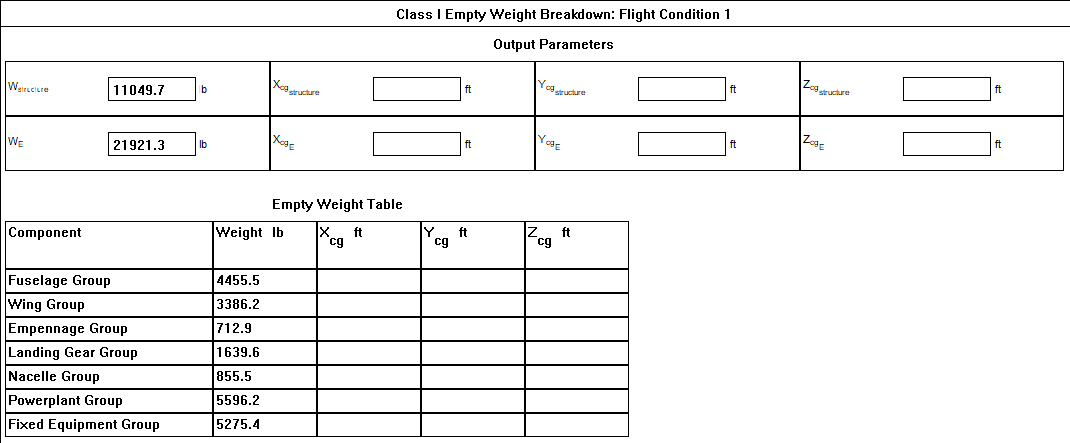
\includegraphics[width=\textwidth]{Report3Printouts/Weight/ComponentWeights_cropped.png}
    \caption{Structural component weight breakdown}
    \label{fig:componentweights}
\end{figure}

\begin{figure}[H]
    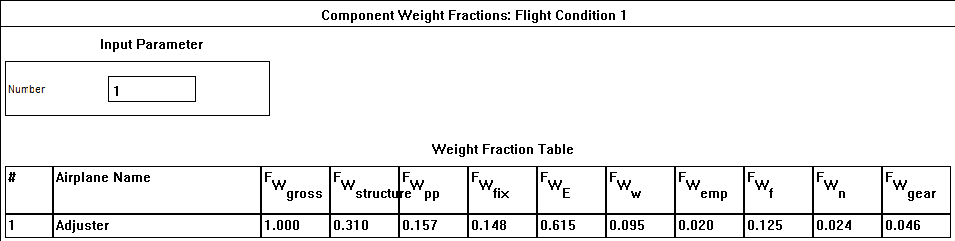
\includegraphics[width=\textwidth]{Report3Printouts/Weight/CustomAirplane_cropped.png}
    \caption{A custom airplane model used for weight allocation in AAA}
    \label{fig:customairplane}
\end{figure}

\begin{figure}[H]
    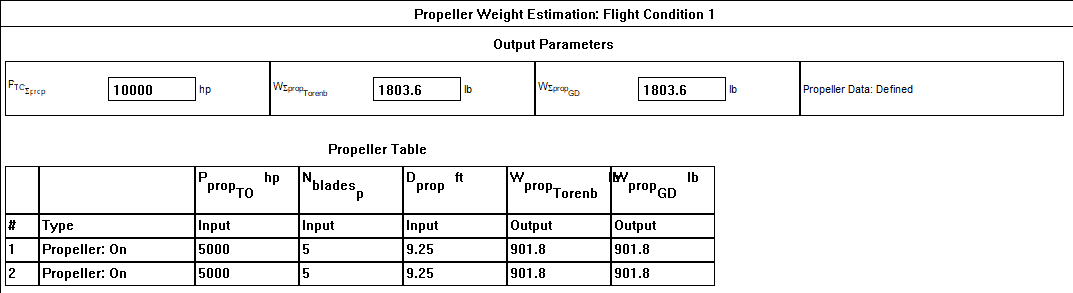
\includegraphics[width=\textwidth]{Report3Printouts/Weight/PropellerWeight_cropped.png}
    \caption{Propeller weights estimates}
    \label{fig:propellerweight}
\end{figure}

\begin{figure}[H]
    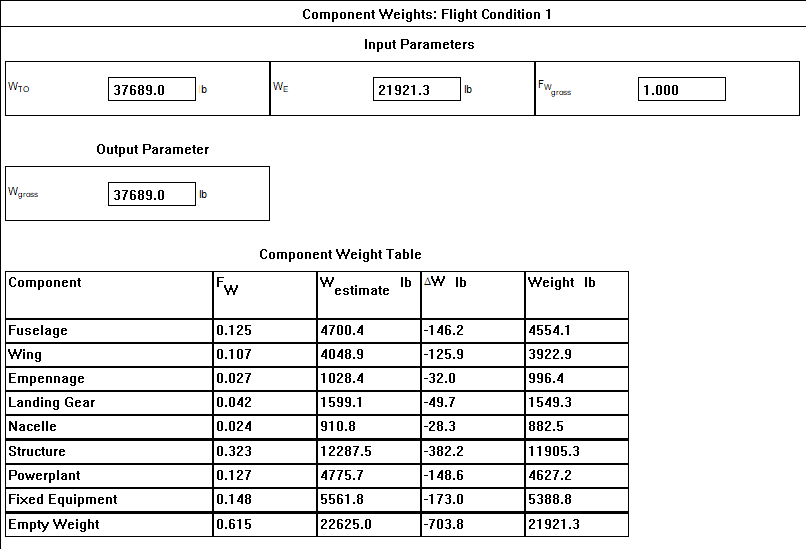
\includegraphics[width=\textwidth]{Report3Printouts/Weight/WeightFractionsInitial_cropped.png}
    \caption{Initial structural weight fractions}
    \label{fig:weightfractionsinitial}
\end{figure}

\begin{figure}[H]
    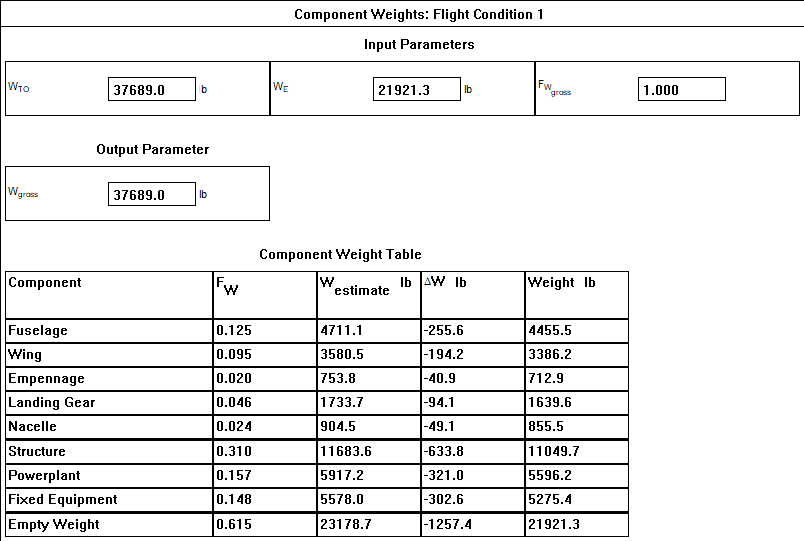
\includegraphics[width=\textwidth]{Report3Printouts/Weight/WeightFractionsFinal_cropped.png}
    \caption{Finalized structural weight fractions}
    \label{fig:weightfractionsfinal}
\end{figure}

\subsection{AAA: Preliminary Balance Analysis}

\begin{figure}[H]
    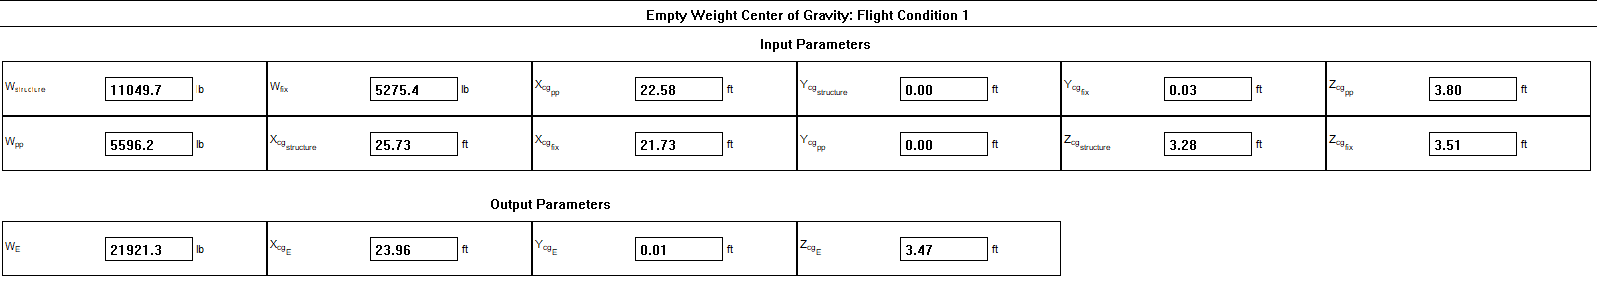
\includegraphics[width=\textwidth]{Report3Printouts/Cg/Cg_Empty_Detailed_Empty_cropped.png}
    \caption{Detailed breakdown of CG components of the empty aircraft}
    \label{fig:cg_detailed_empty}
\end{figure}

\begin{figure}[H]
    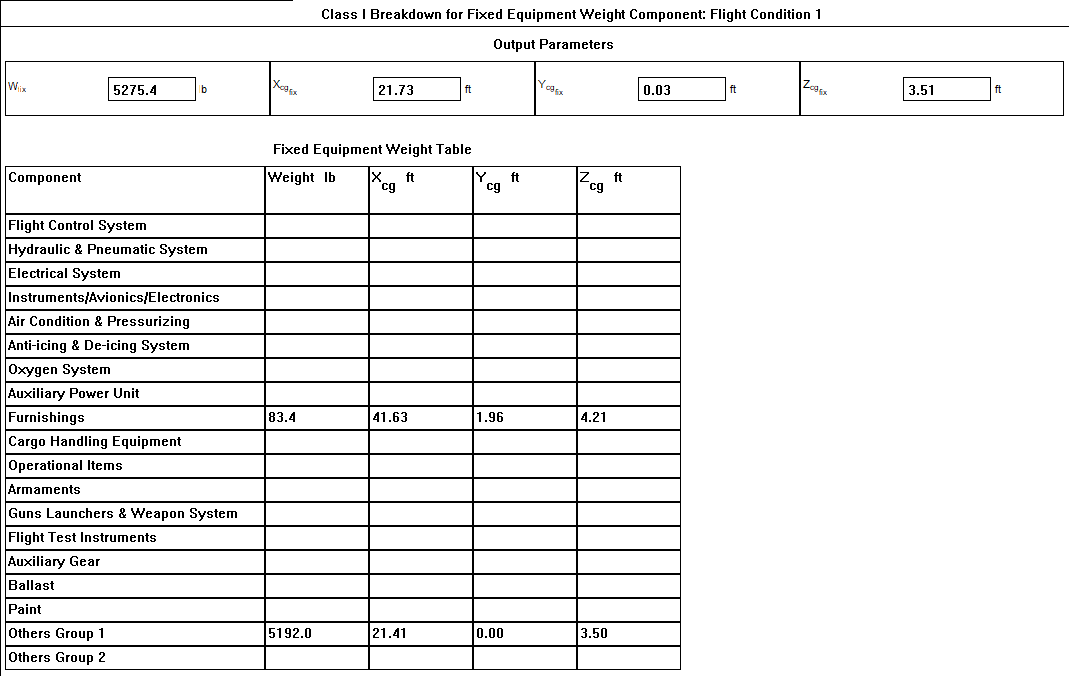
\includegraphics[width=\textwidth]{Report3Printouts/Cg/Cg_Empty_Detailed_FixedEquipment_cropped.png}
    \caption{Detailed breakdown of CG and weight of the fixed equipment}
    \label{fig:cg_empty_detailed_fixedequipment}
\end{figure}

\begin{figure}[H]
    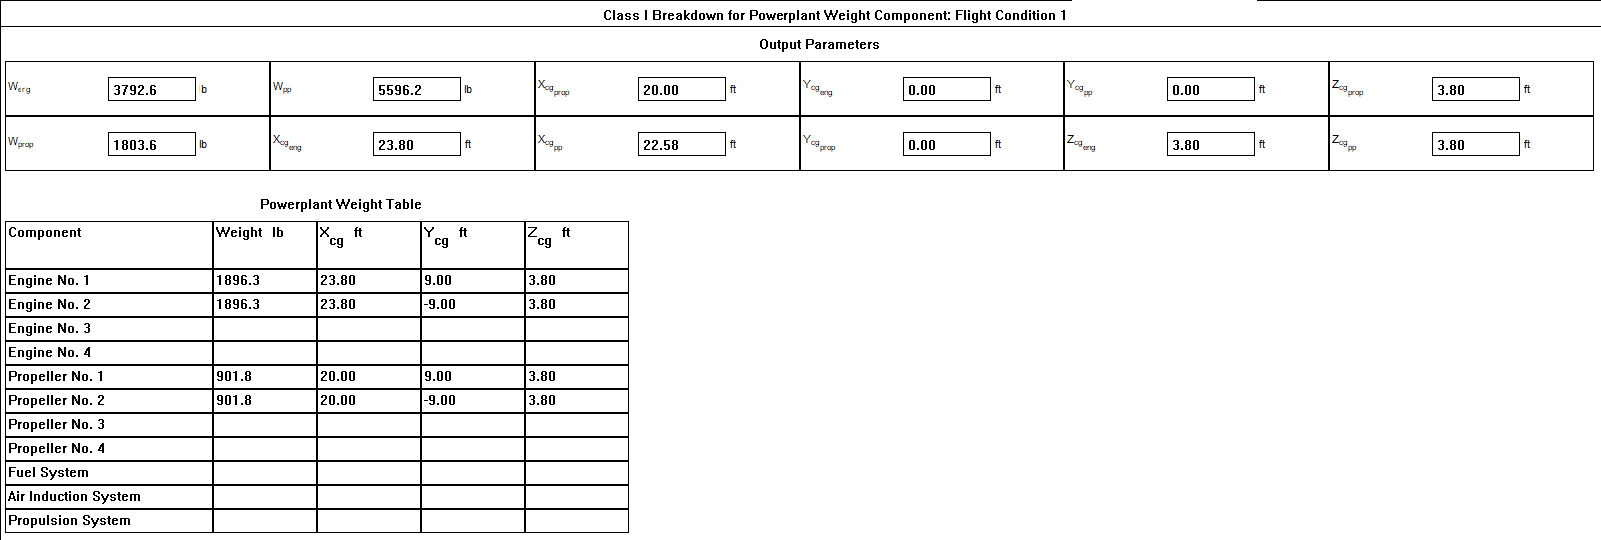
\includegraphics[width=\textwidth]{Report3Printouts/Cg/Cg_Empty_Detailed_Powerplant_cropped.png}
    \caption{Powerplant CG breakdown}
    \label{fig:cg_empty_detailed_powerplant}
\end{figure}


\begin{figure}[H]
    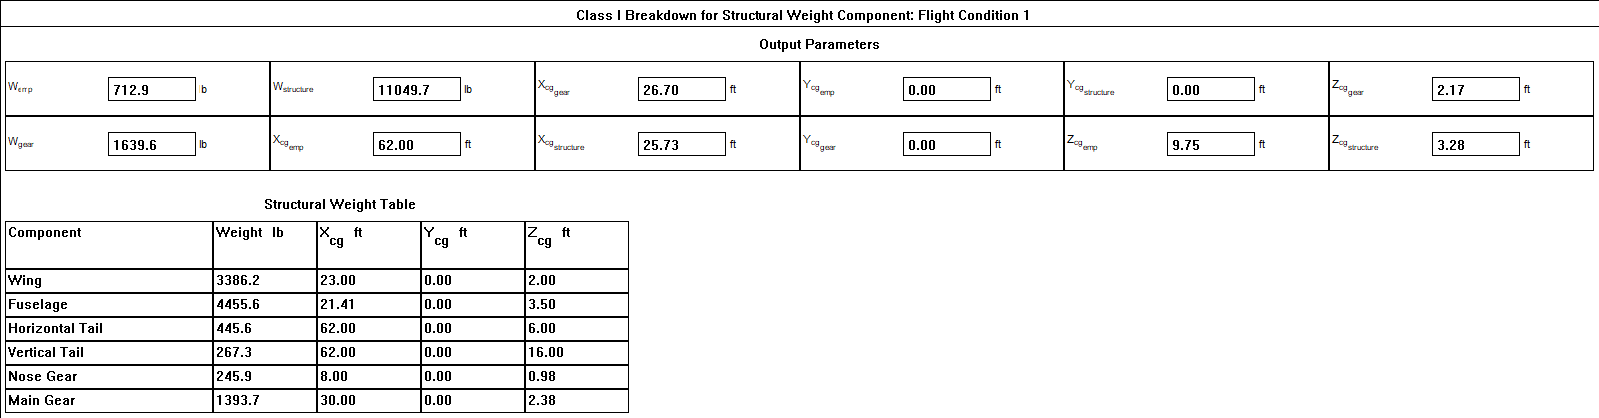
\includegraphics[width=\textwidth]{Report3Printouts/Cg/Cg_Empty_Detailed_Structure_cropped.png}
    \caption{Structure CG breakdown}
    \label{fig:cg_empty_detailed_structure}
\end{figure}


\begin{figure}[H]
    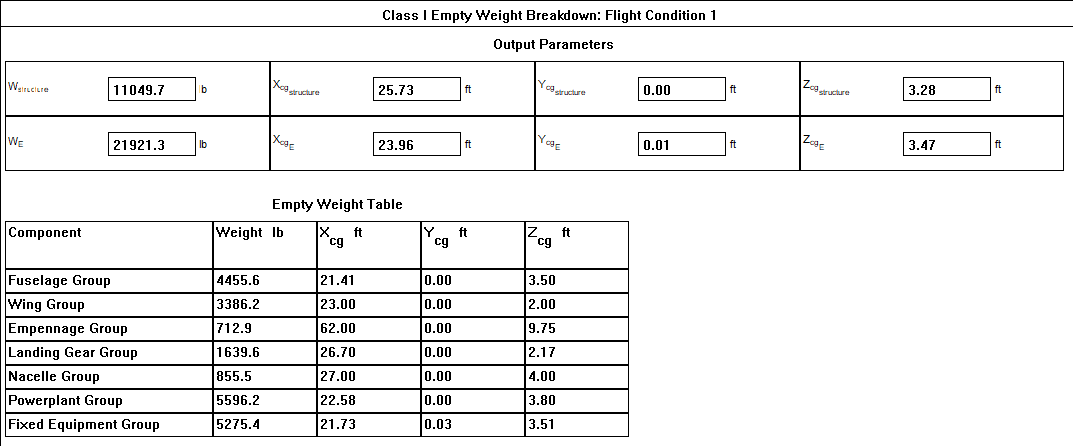
\includegraphics[width=\textwidth]{Report3Printouts/Cg/Cg_Empty_Fractions_cropped.png}
    \caption{Equipment group CG breakdown}
    \label{fig:cg_empty_fractions}
\end{figure}


\begin{figure}[H]
    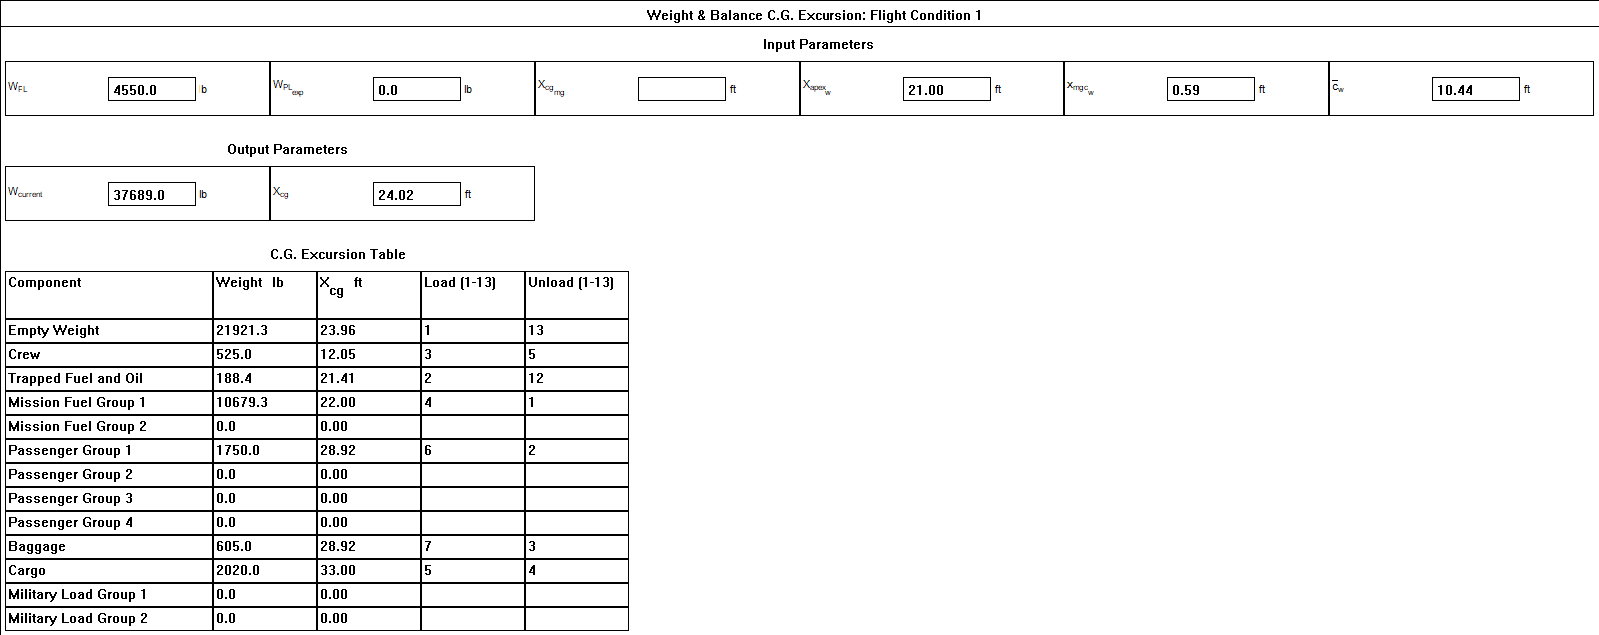
\includegraphics[width=\textwidth]{Report3Printouts/Cg/Cg_Excursion_cropped.png}
    \caption{CG excursion ordering}
    \label{fig:cg_excursion}
\end{figure}

\begin{figure}[H]
    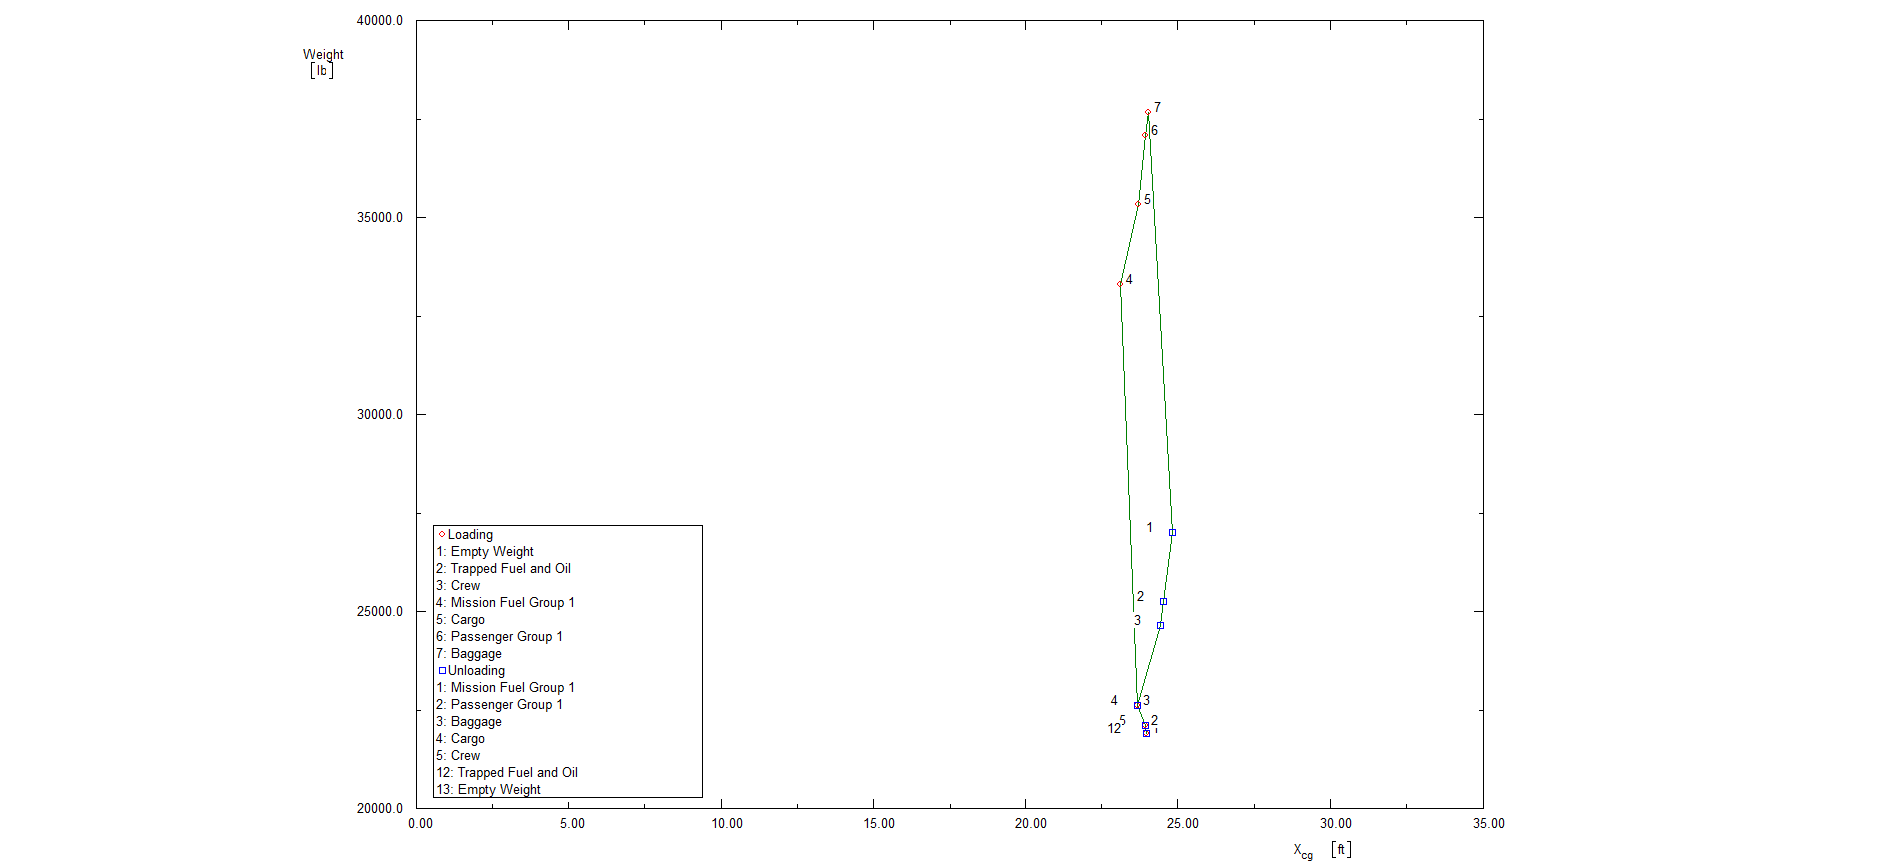
\includegraphics[width=\textwidth]{Report3Printouts/Cg/Cg_Excursion_Plot_cropped.png}
    \caption{Plot of CG excursion}
    \label{fig:cg_excursion_plot}
\end{figure}

\begin{figure}[H]
    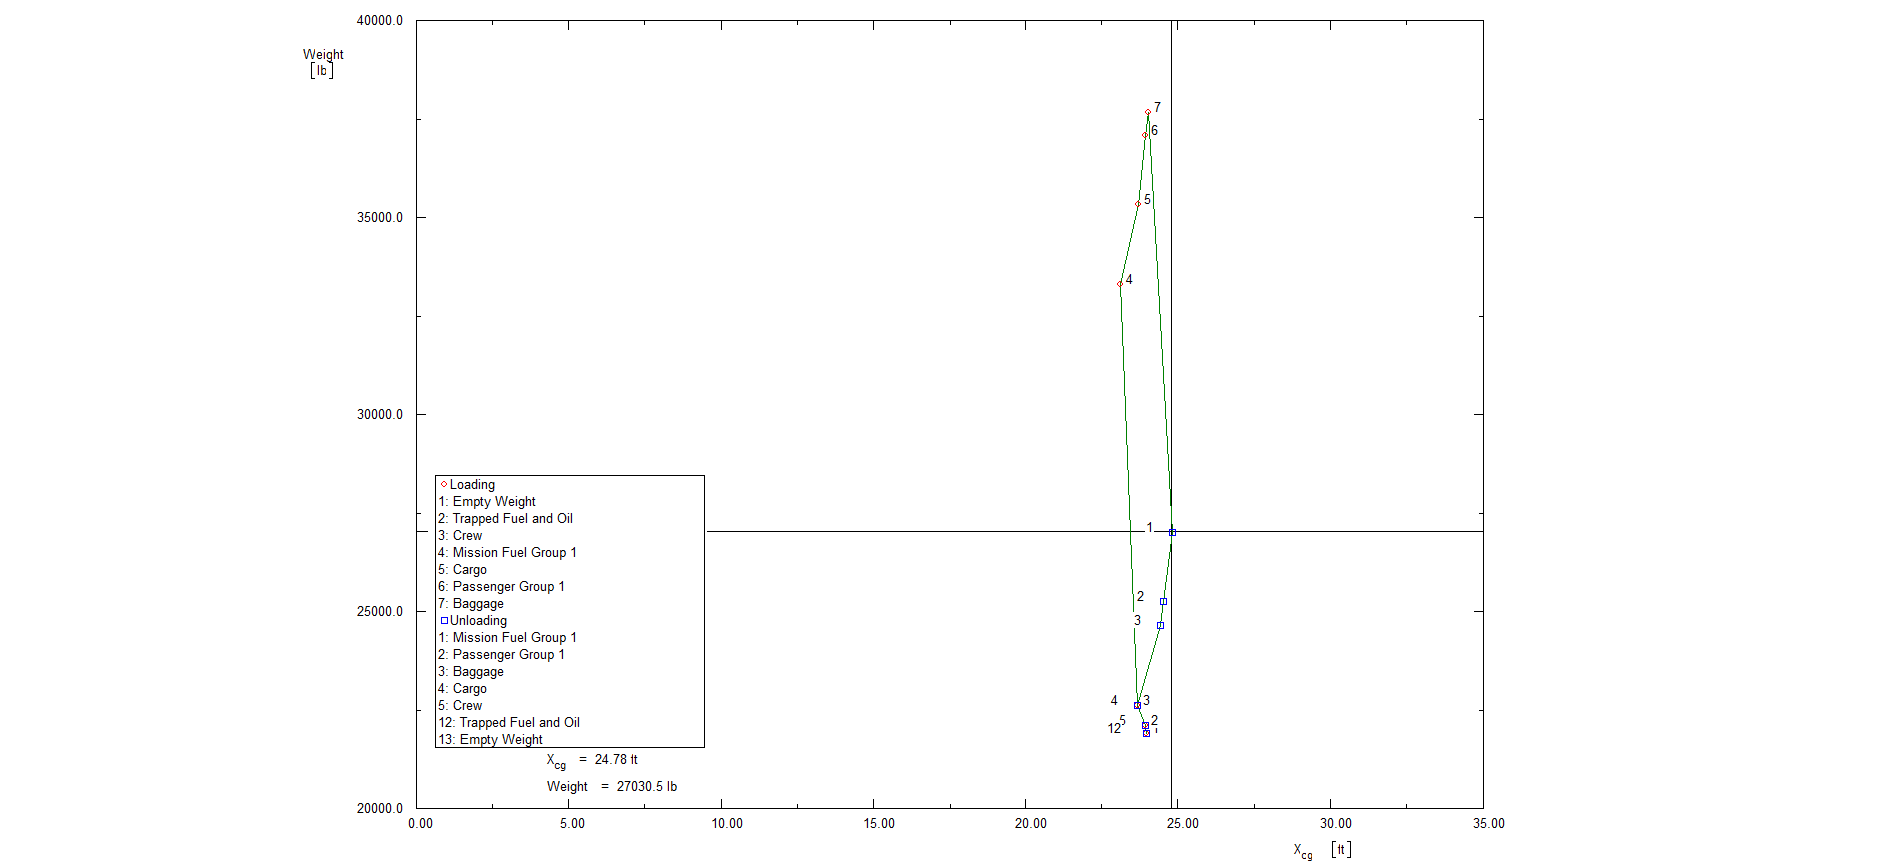
\includegraphics[width=\textwidth]{Report3Printouts/Cg/Cg_excursion_plot_mostaft_cropped.png}
    \caption{Plot of CG excursion with most aft point marked}
    \label{fig:cg_excursion_plot_mostaft}
\end{figure}


\begin{figure}[H]
    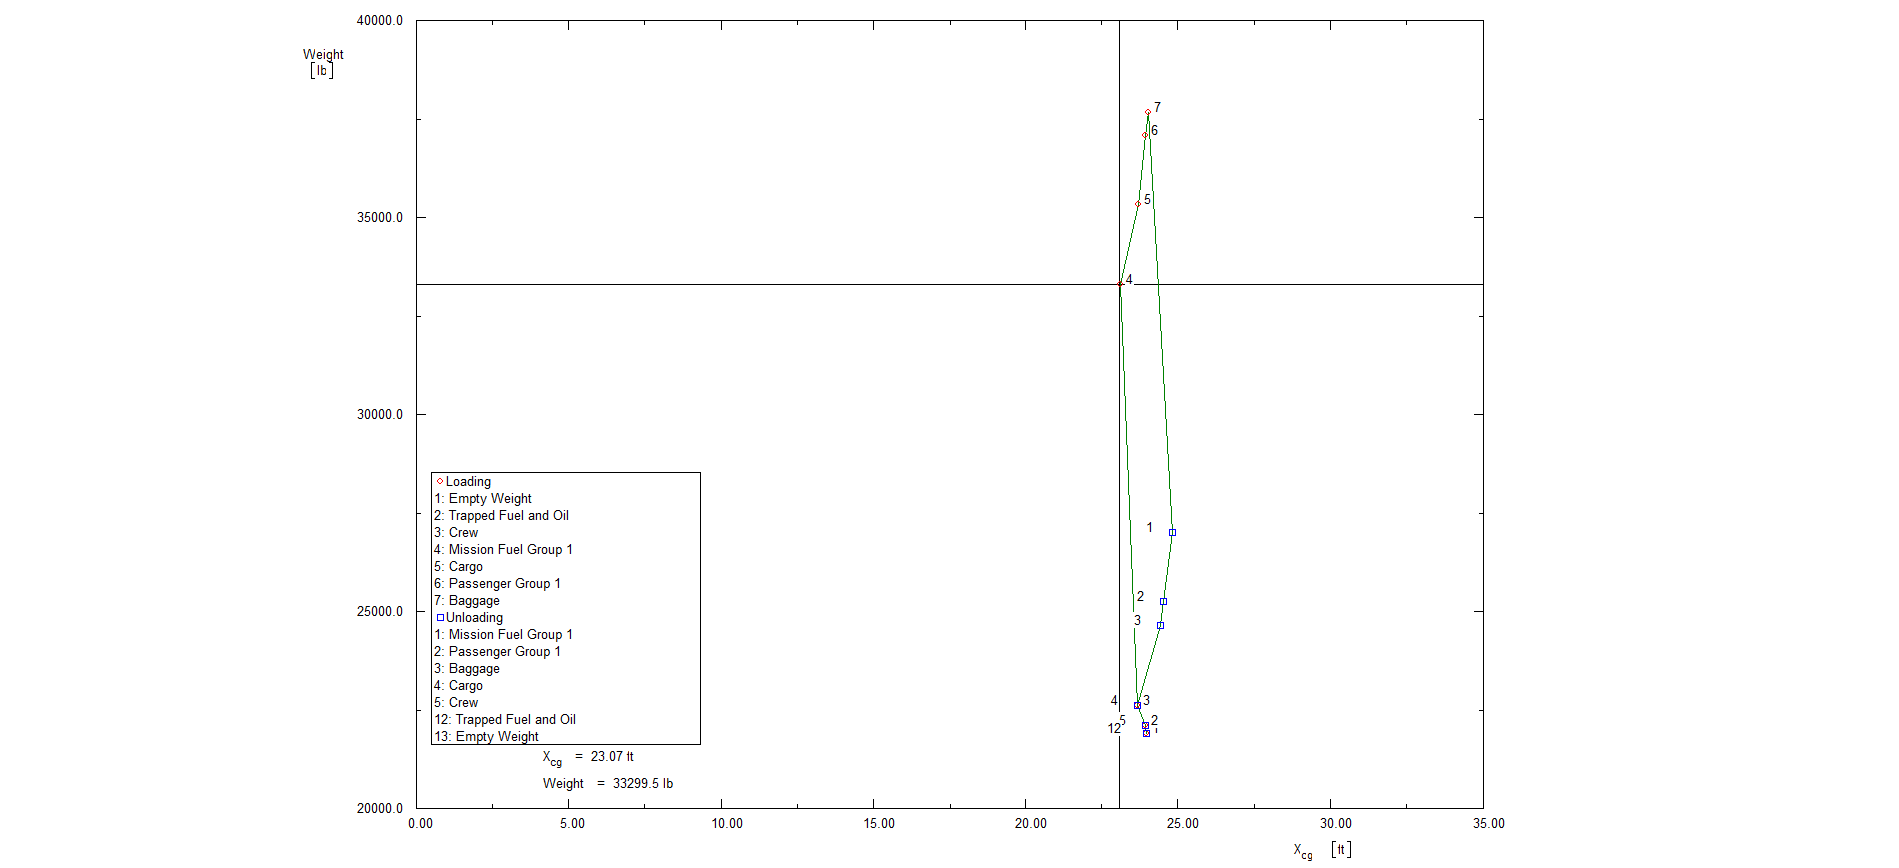
\includegraphics[width=\textwidth]{Report3Printouts/Cg/Cg_excursion_plot_mostforward_cropped.png}
    \caption{Plot of CG excursion with most forward point marked}
    \label{fig:cg_excursion_plot_mosforward}
\end{figure}

\begin{figure}[H]
    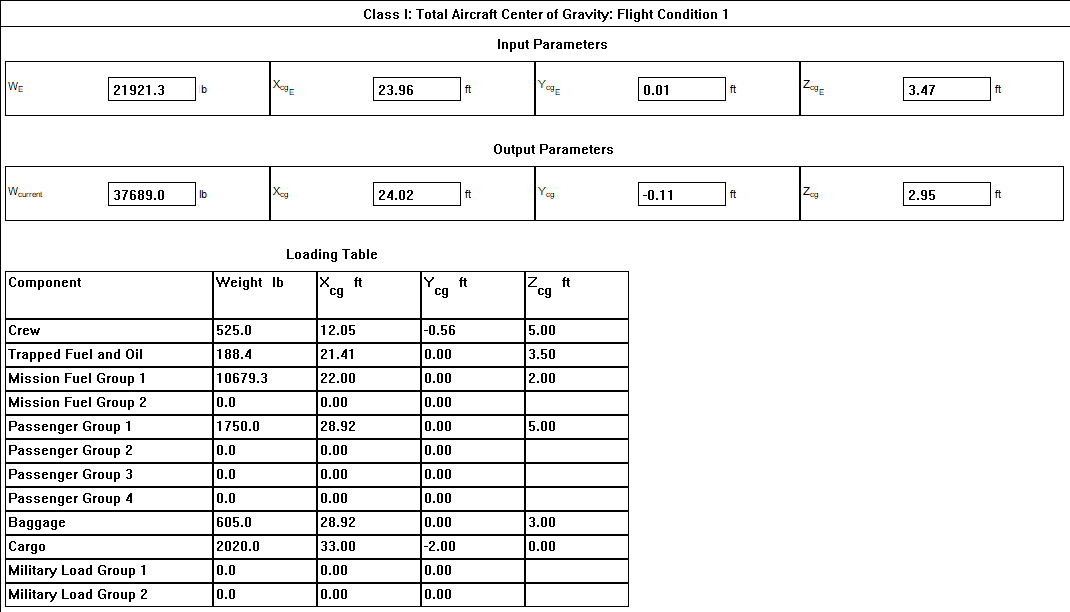
\includegraphics[width=\textwidth]{Report3Printouts/Cg/Cg_TotalAircraft_cropped.png}
    \caption{Fully loaded aircraft CG breakdown}
    \label{fig:cg_totalaircraft}
\end{figure}

\subsection{AAA: Empennage Layout Design}

\begin{figure}[H]
    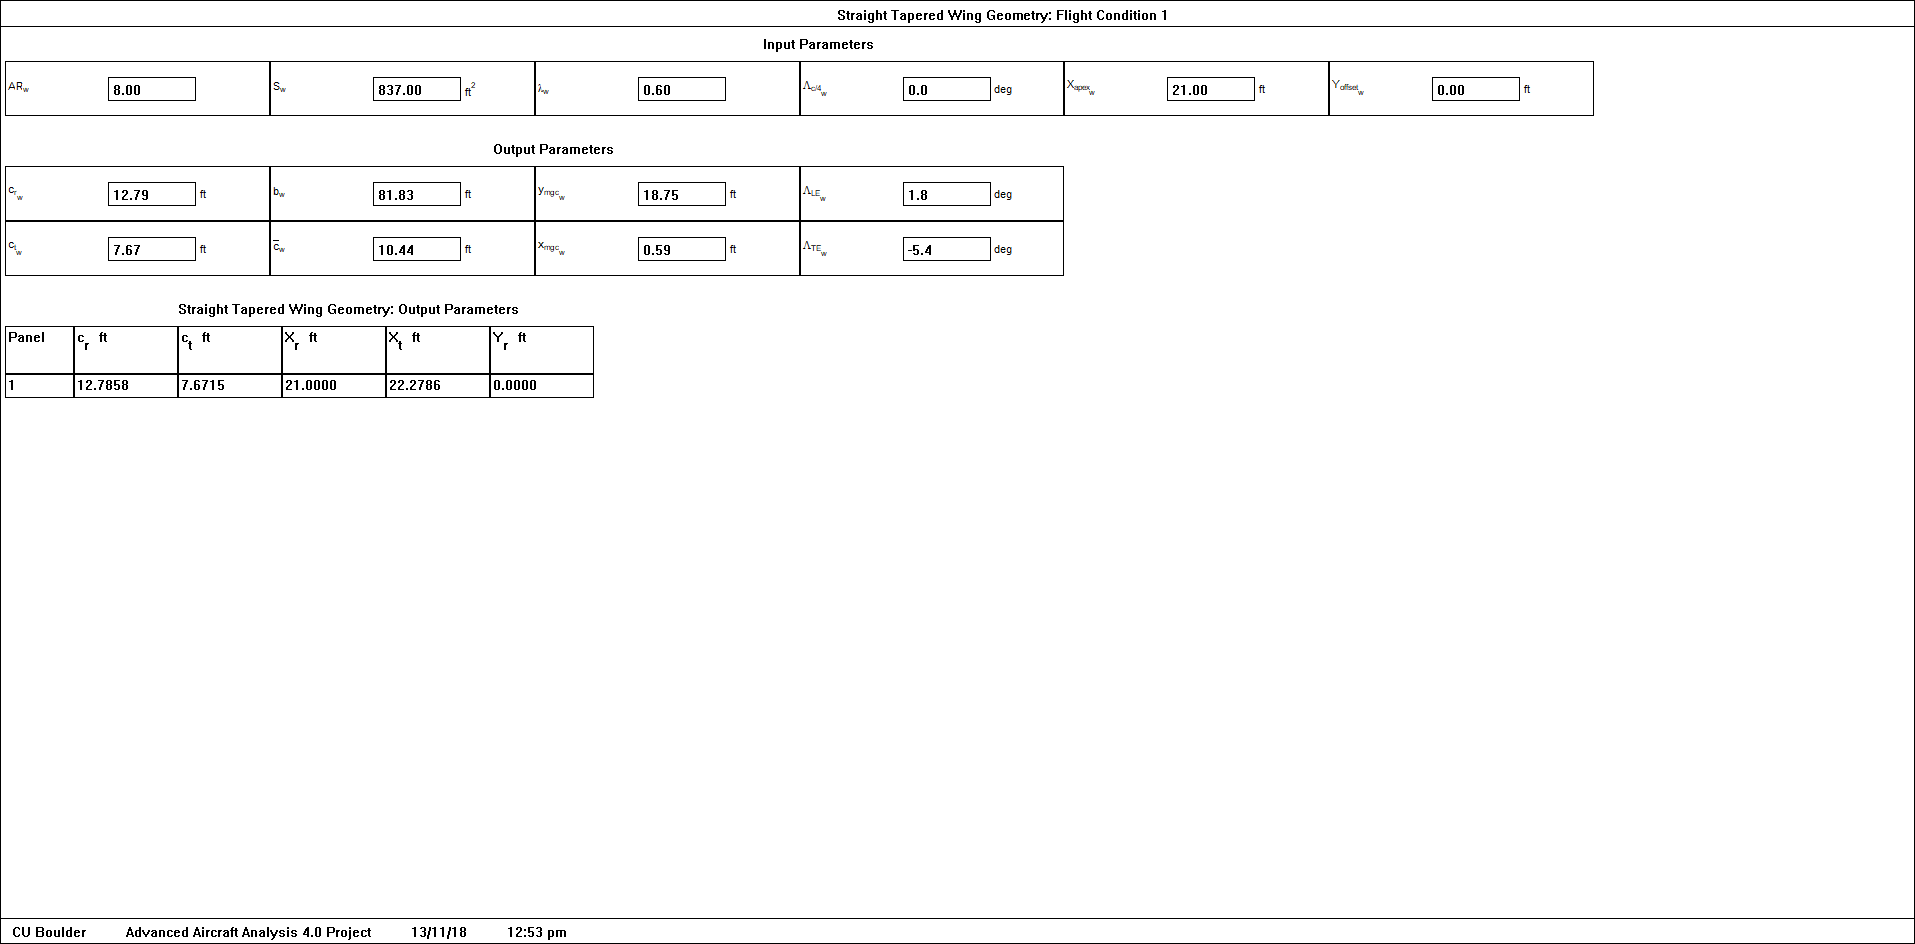
\includegraphics[width=\textwidth]{Report3Printouts/changedwing.png}
    \caption{Wing layout, with adjusted apex location}
    \label{fig:changedwing}
\end{figure}

\begin{figure}[H]
    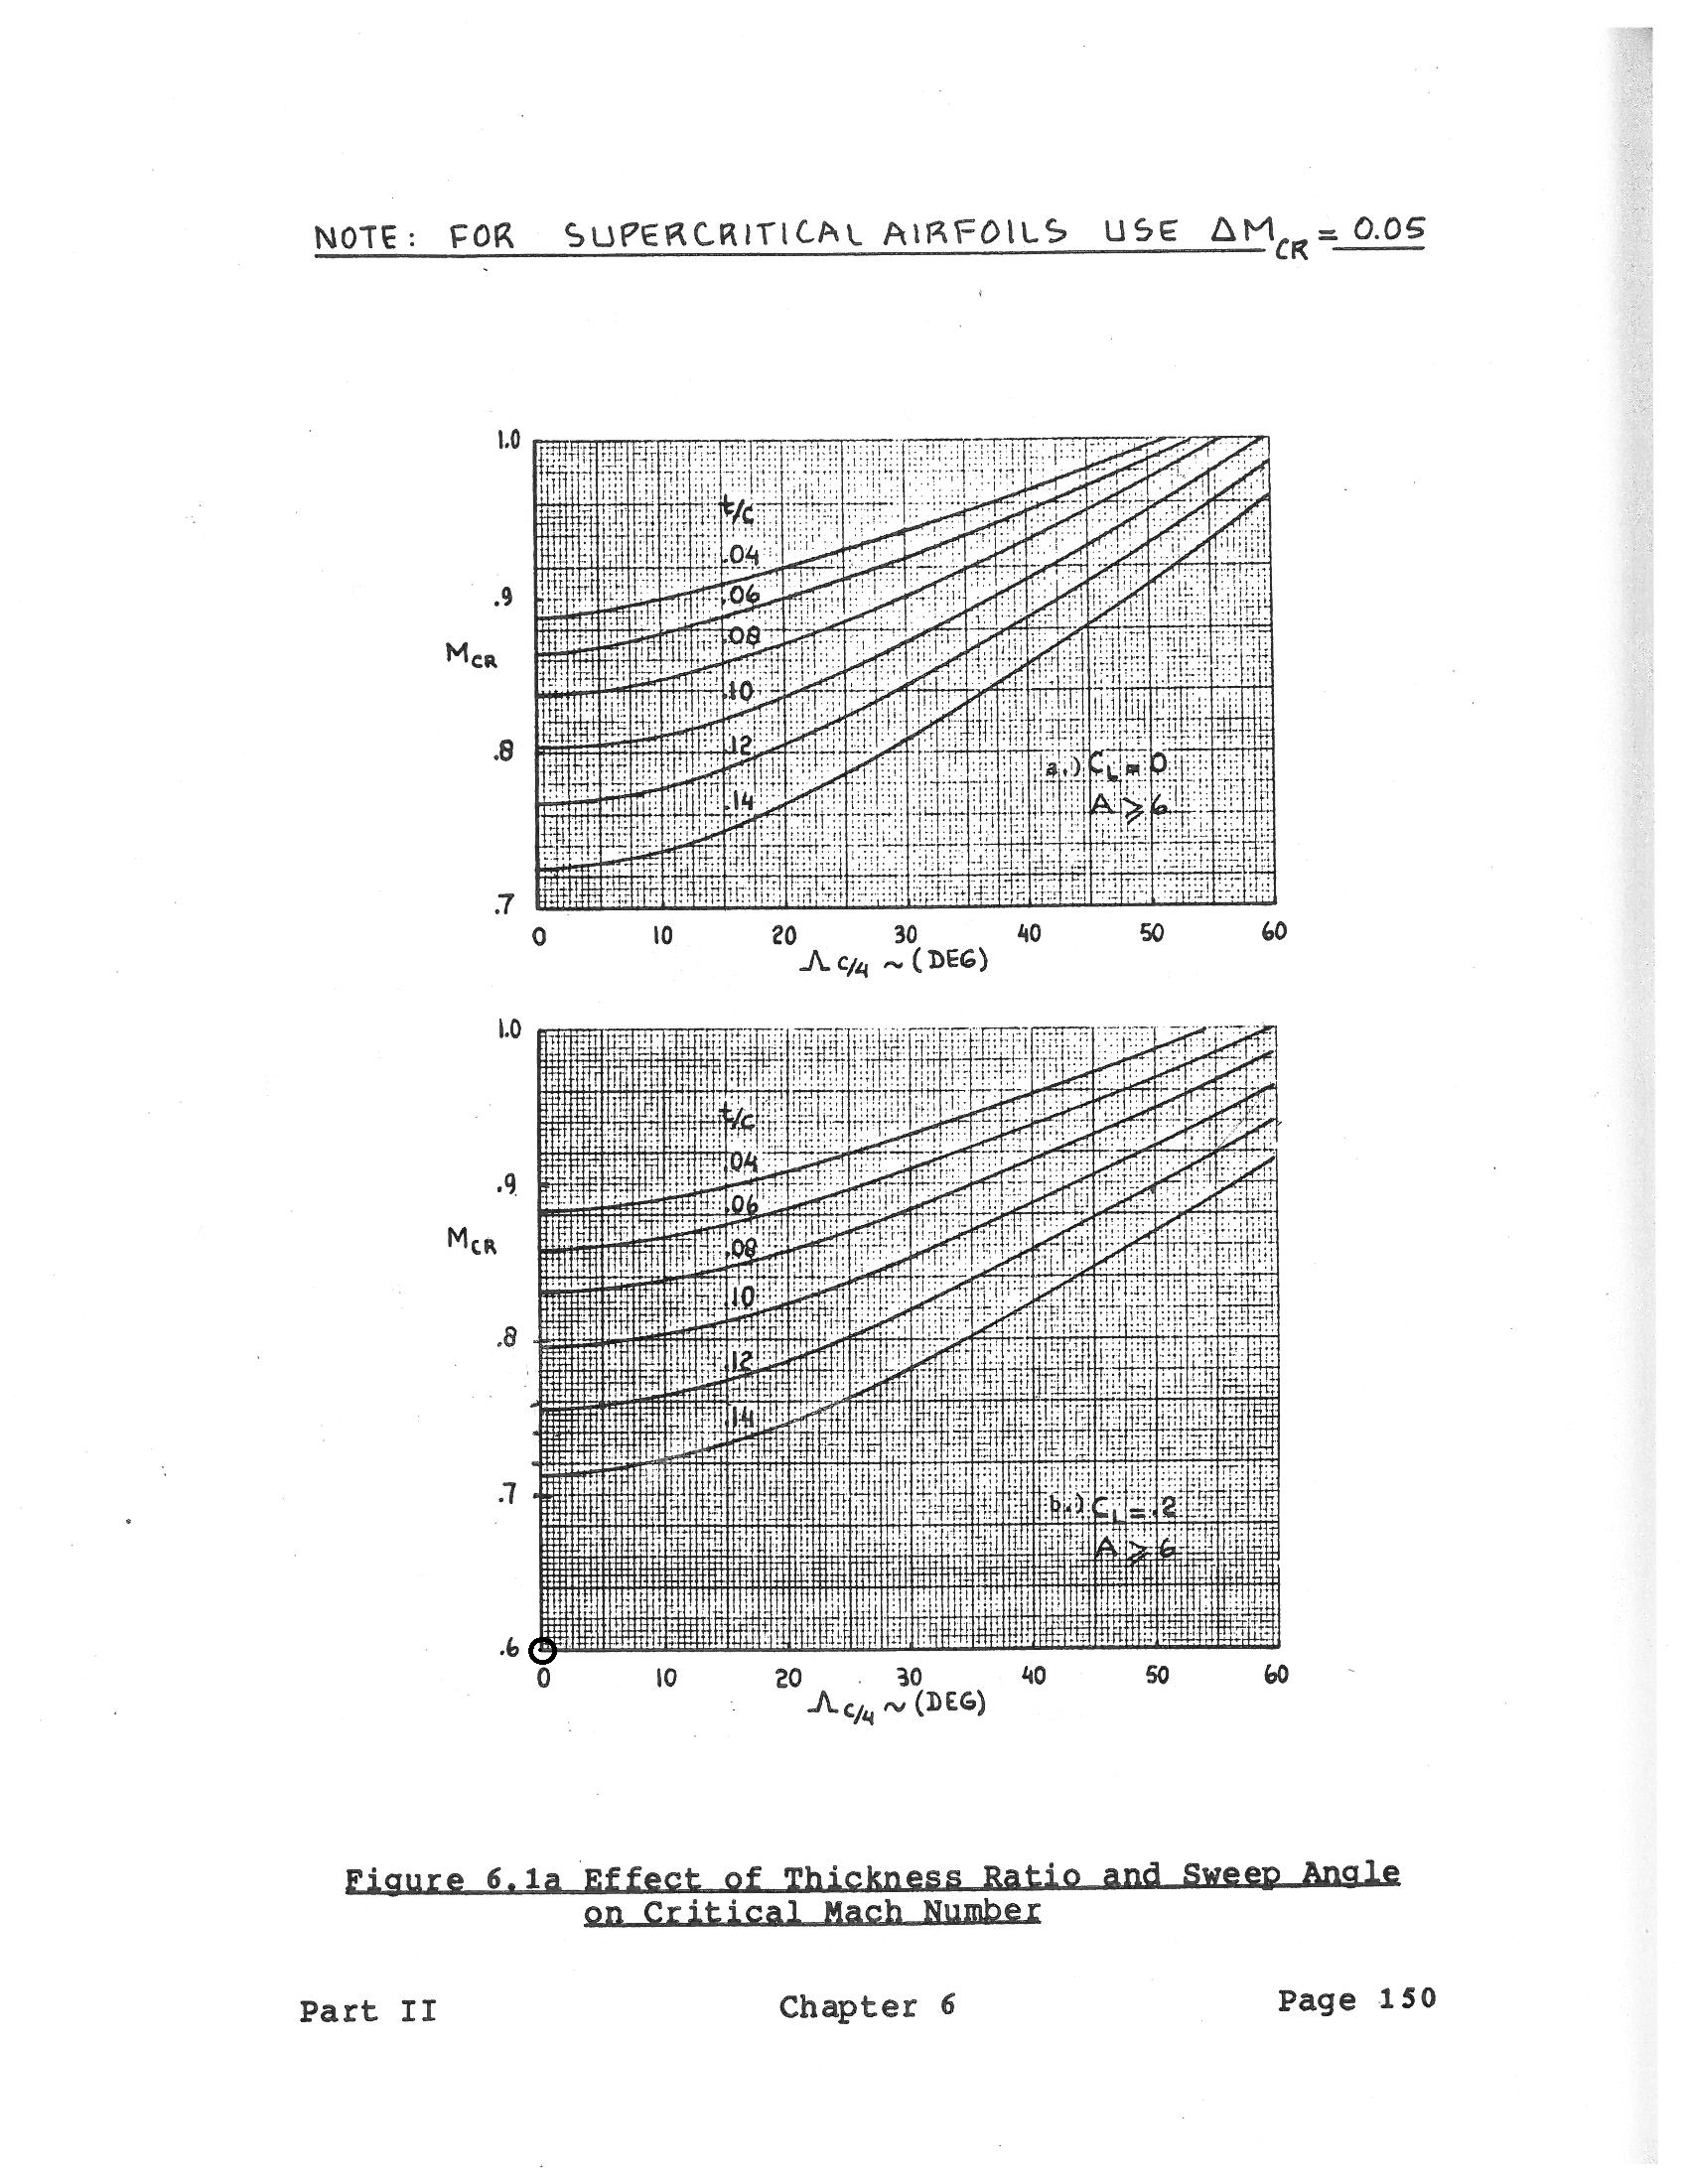
\includegraphics[width=\textwidth]{plots/Mcr_check.png}
    \label{fig:critical_mach_check}
    \caption{Critical Mach number checks for shockwave formation on an airfoil}
\end{figure}

\begin{figure}[H]
    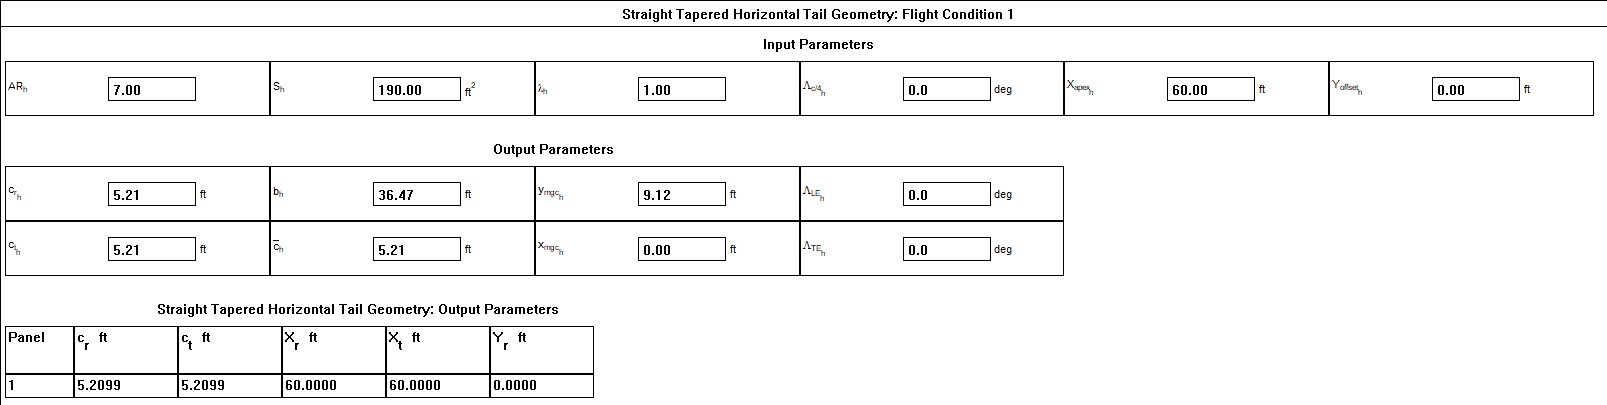
\includegraphics[width=\textwidth]{Report3Printouts/Empannage/Horizontal_geometry_cropped.png}
    \caption{Horizontal stabilizer sizing}
    \label{fig:horizontal_geometry}
\end{figure}

\begin{figure}[H]
    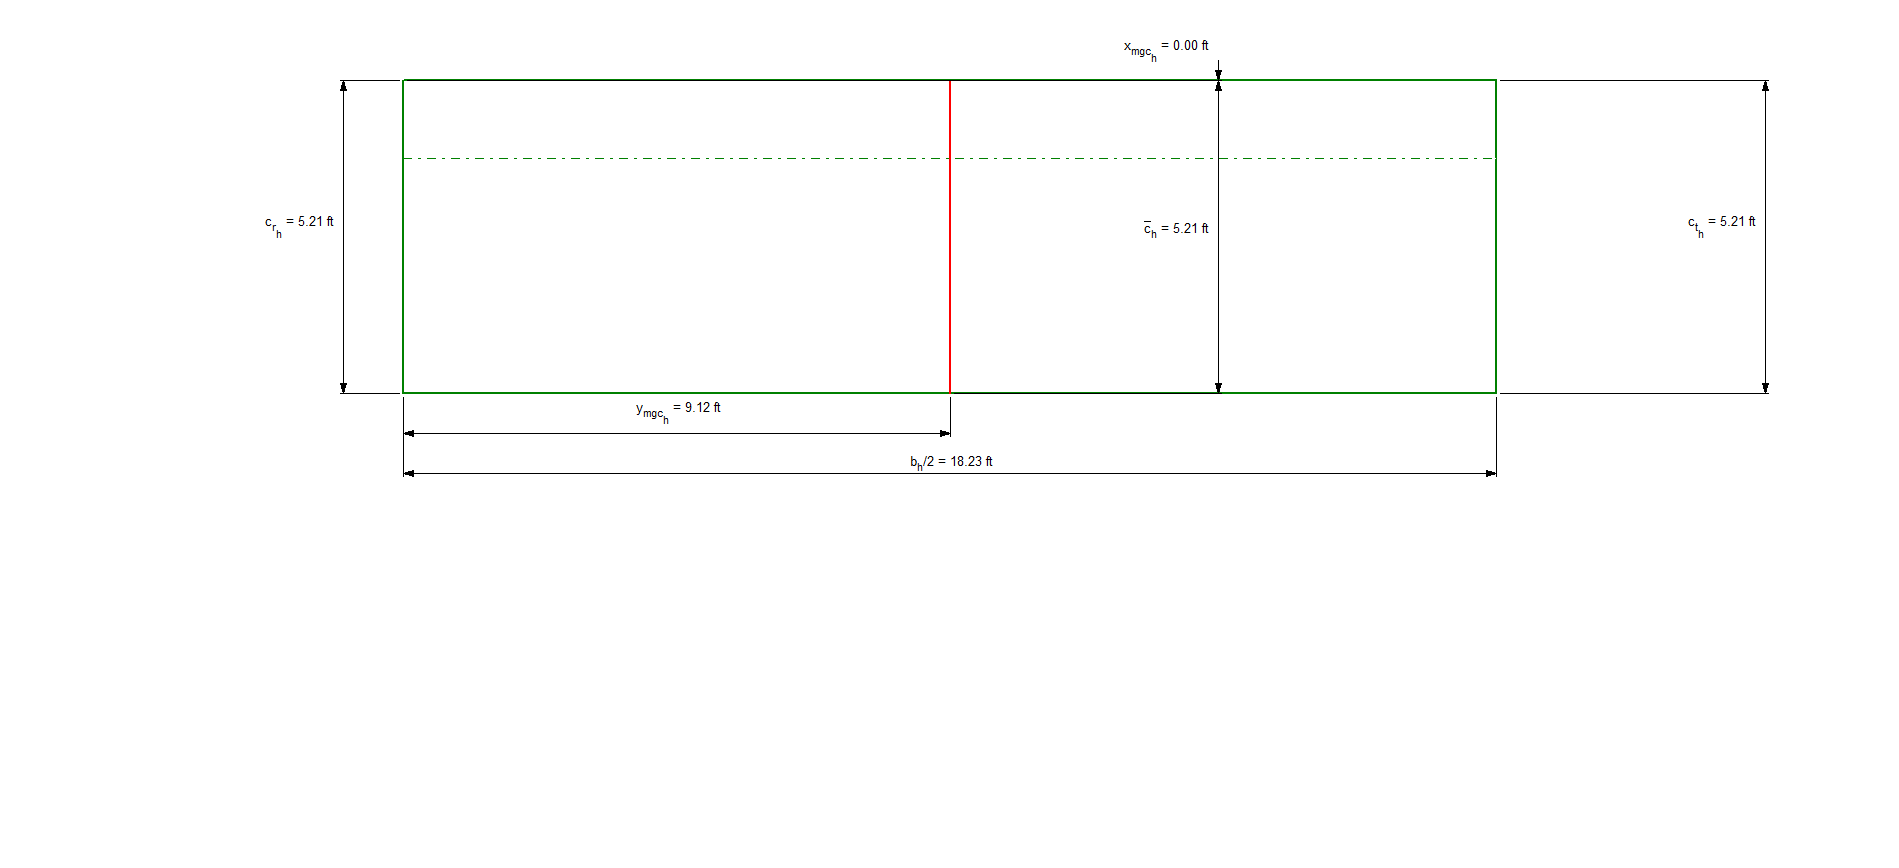
\includegraphics[width=\textwidth]{Report3Printouts/Empannage/Horizontal_geometry_plot.png}
    \caption{Horizontal stabilizer layout}
    \label{fig:horizontal_geometry_plot}
\end{figure}

\begin{figure}[H]
    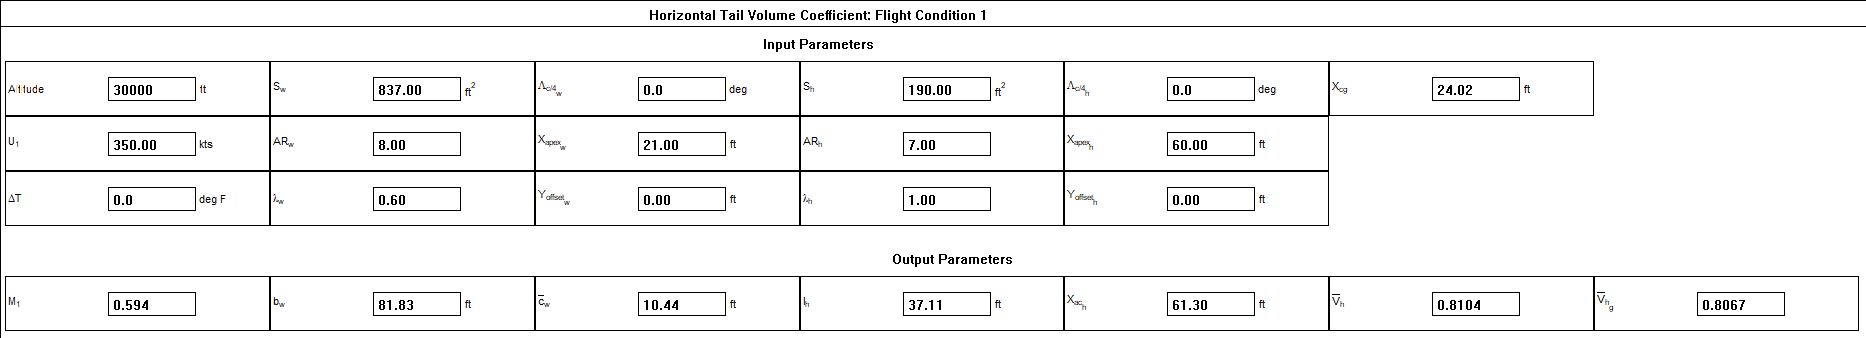
\includegraphics[width=\textwidth]{Report3Printouts/Empannage/Horizontal_volumeratio_cropped.png}
    \caption{Horizontal tail volume coefficient calculations}
    \label{fig:horizontal_volumeratio}
\end{figure}

\begin{figure}[H]
    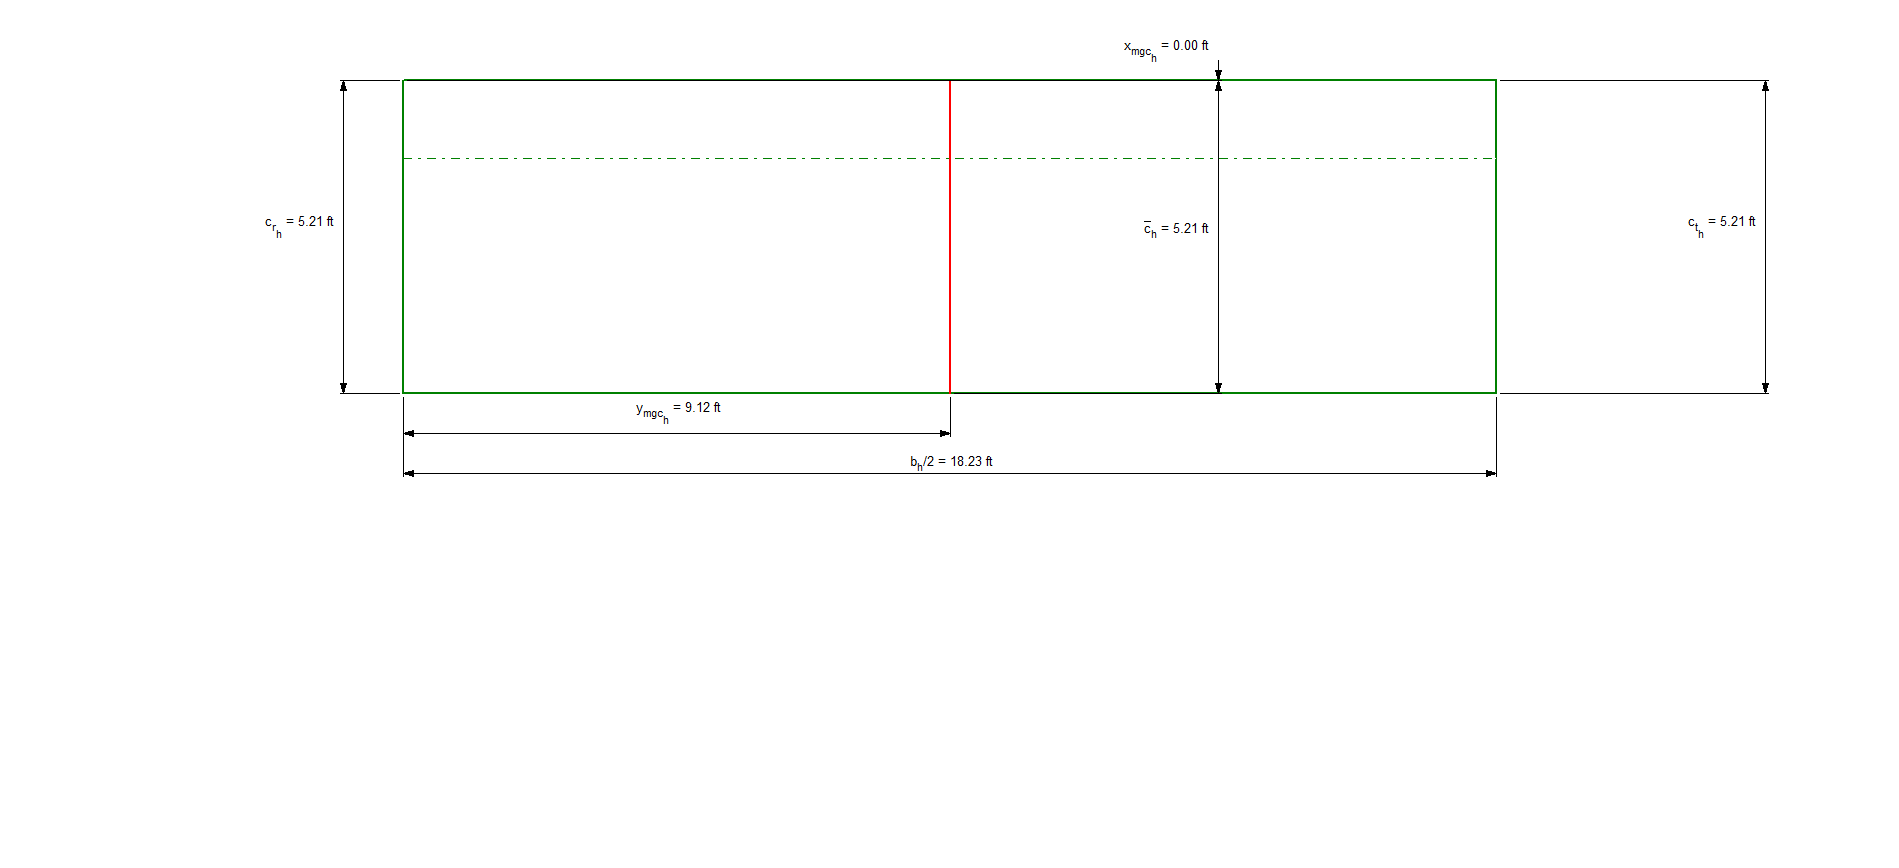
\includegraphics[width=\textwidth]{Report3Printouts/Empannage/Horizontal_volumeratio_plot.png}
    \caption{Horizontal stabilizer with aerodynamic center shown}
    \label{fig:horizontal_volumeratio_plot}
\end{figure}

\begin{figure}[H]
    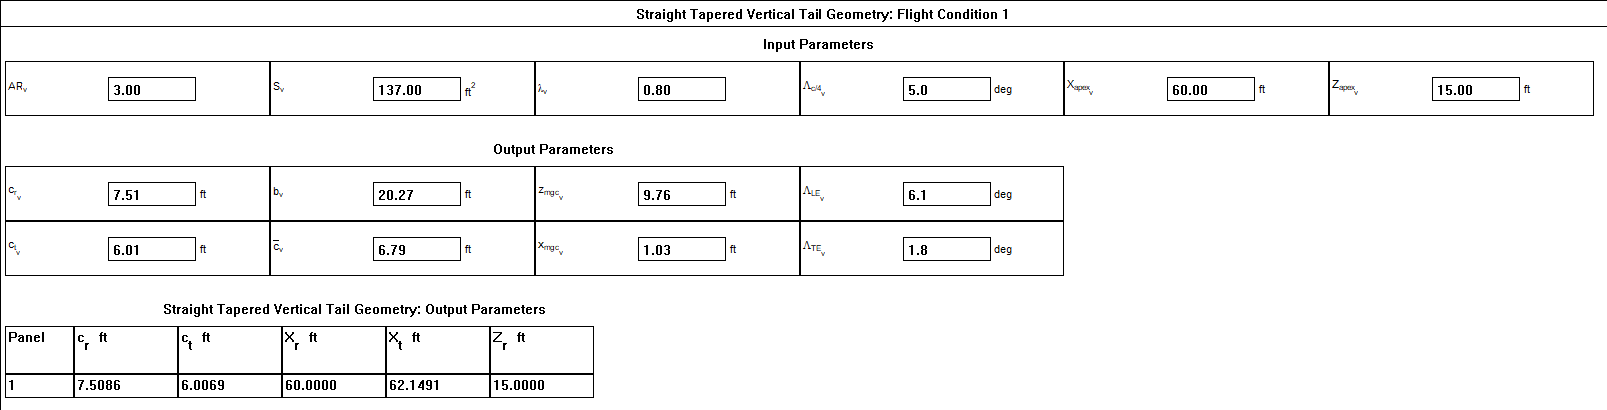
\includegraphics[width=\textwidth]{Report3Printouts/Empannage/Vertical_geometry_cropped.png}
    \caption{Vertical stabilizer sizing}
    \label{fig:vertical_geometry}
\end{figure}

\begin{figure}[H]
    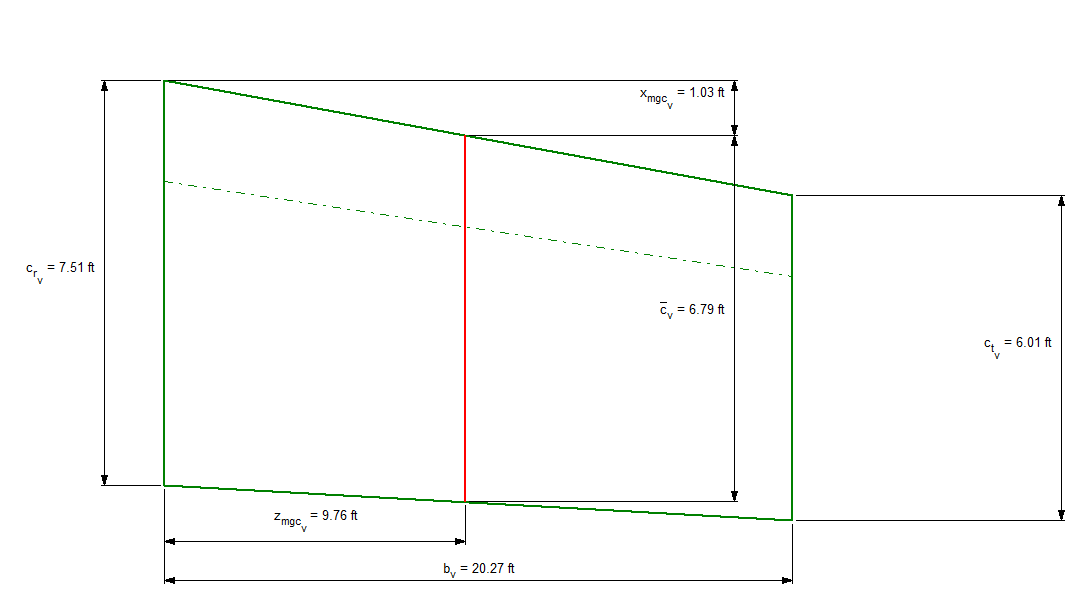
\includegraphics[width=\textwidth]{Report3Printouts/Empannage/Vertical_geometry_plot.png}
    \caption{Vertical stabilizer layout}
    \label{fig:vertical_geometry_plot}
\end{figure}

\begin{figure}[H]
    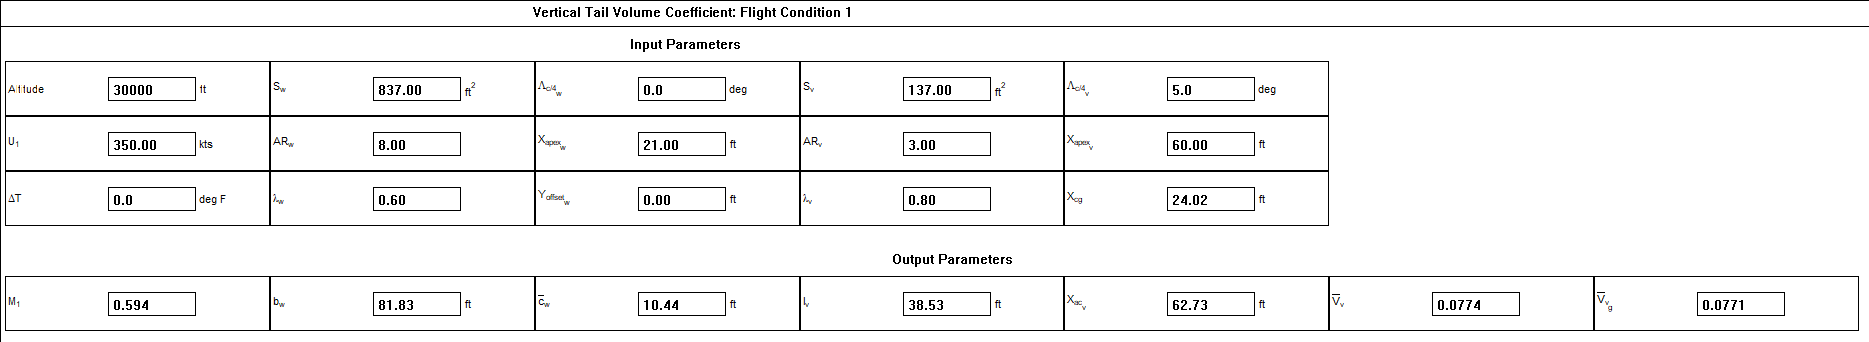
\includegraphics[width=\textwidth]{Report3Printouts/Empannage/Vertical_volumeratio_cropped.png}
    \caption{Vertical stabilizer volume ratio calculation}
    \label{fig:vertical_volumeratio}
\end{figure}

\begin{figure}[H]
    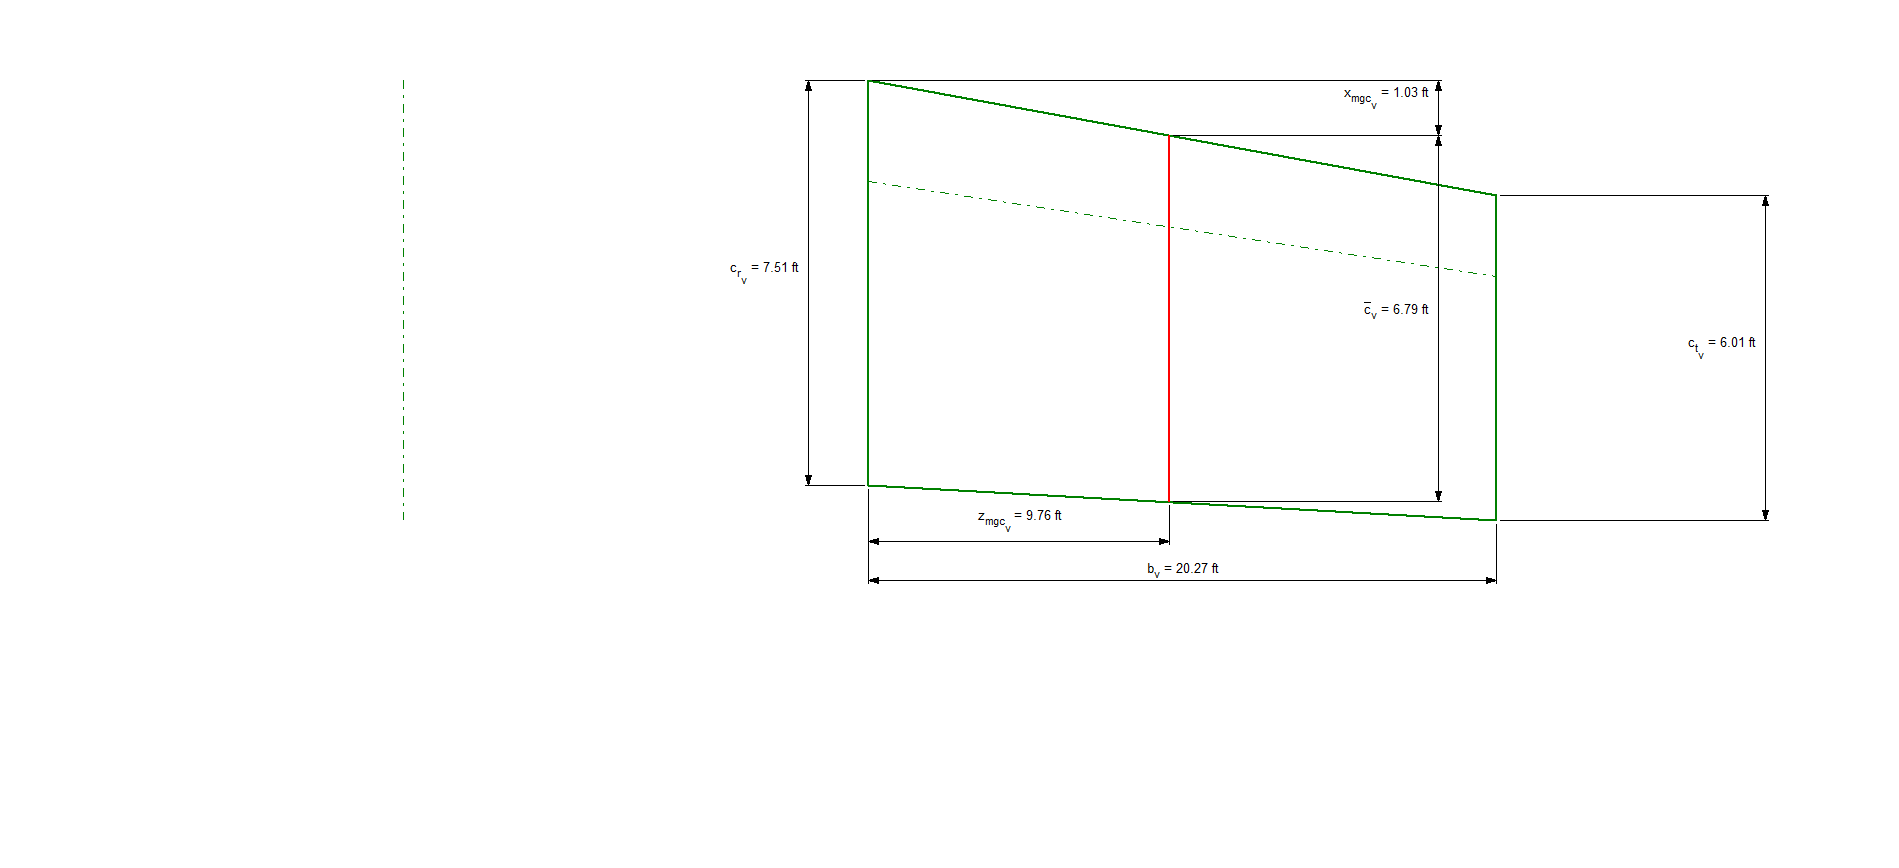
\includegraphics[width=\textwidth]{Report3Printouts/Empannage/Vertical_volumeratio_plot.png}
    \caption{Vertical stabilizer with aerodynamic center shown}
    \label{fig:vertical_volumeratio_plot}
\end{figure}

\subsection{AAA: Control Surface Layout Design}
\begin{figure}[H]
    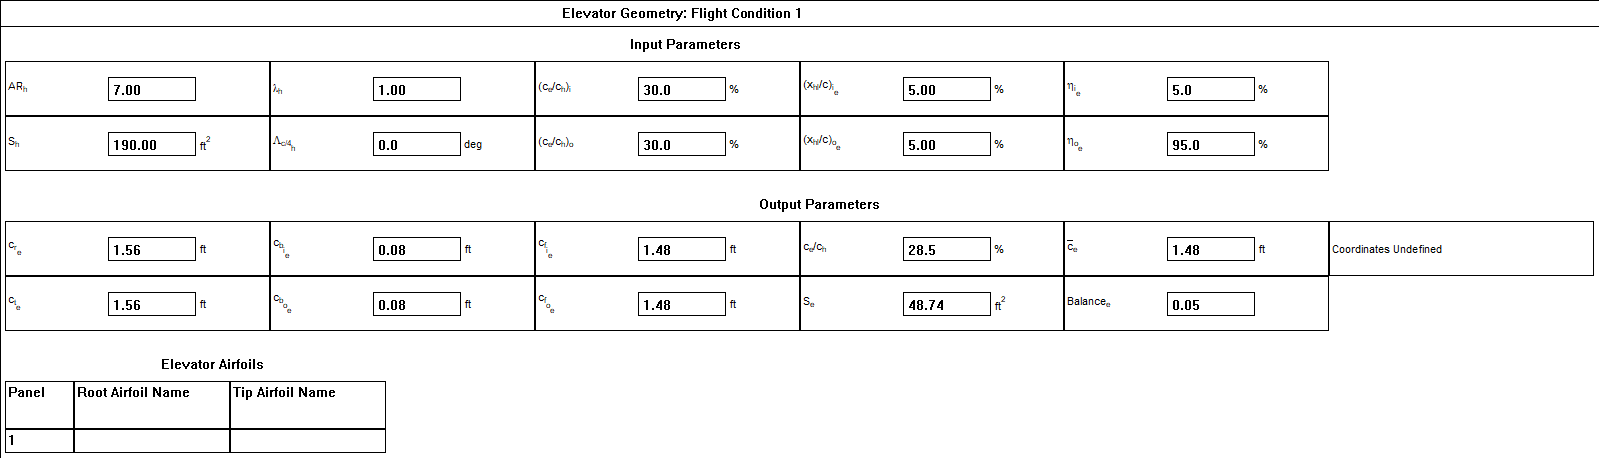
\includegraphics[width=\textwidth]{Report3Printouts/Empannage/Horizontal_elevator_cropped.png}
    \caption{Elevator control surface sizing}
    \label{fig:horizontal_elevator}
\end{figure}

\begin{figure}[H]
    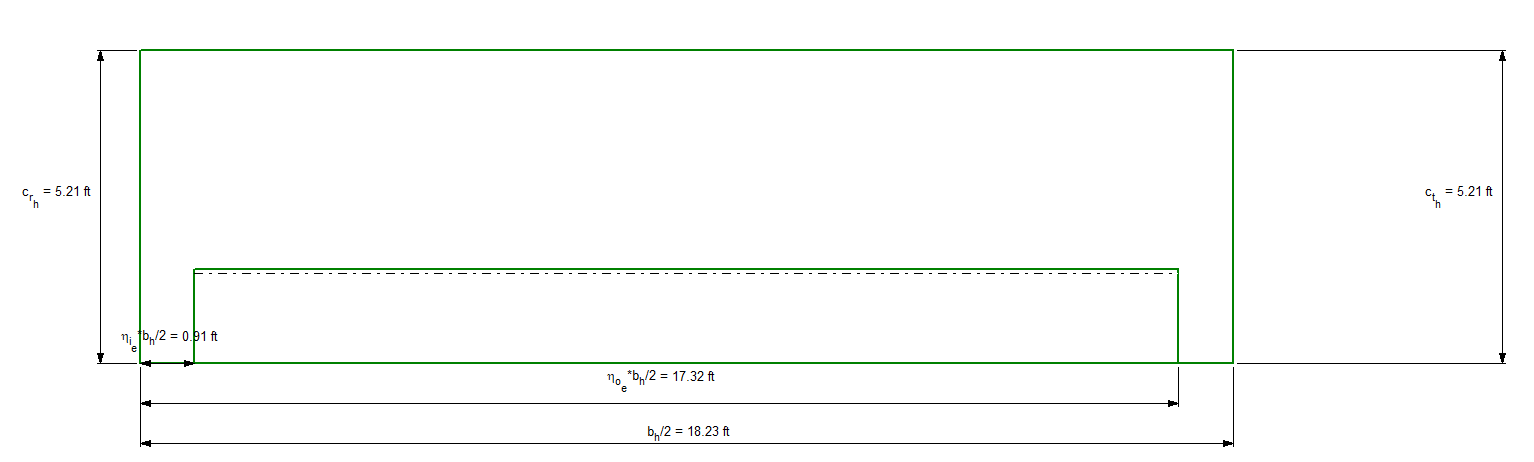
\includegraphics[width=\textwidth]{Report3Printouts/Empannage/Horizontal_elevator_plot.png}
    \caption{Elevator and horizontal stabilizer layout}
    \label{fig:horizontal_elevator_plot}
\end{figure}

\begin{figure}[H]
    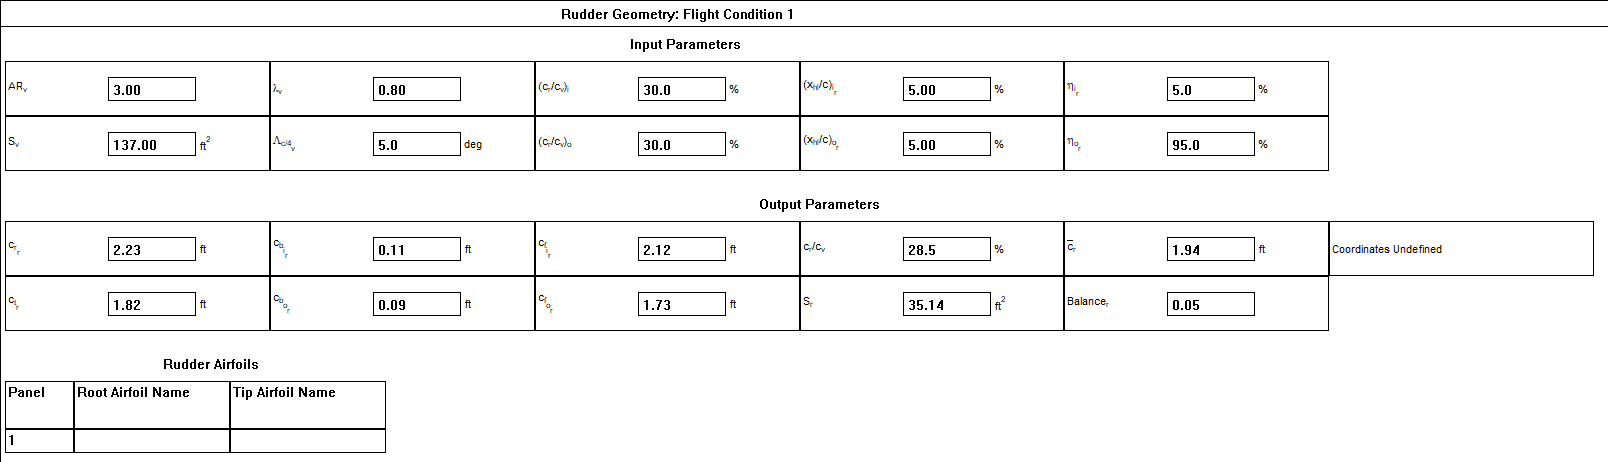
\includegraphics[width=\textwidth]{Report3Printouts/Empannage/Vertical_rudder_cropped.png}
    \caption{Rudder sizing}
    \label{fig:vertical_rudder}
\end{figure}

\begin{figure}[H]
    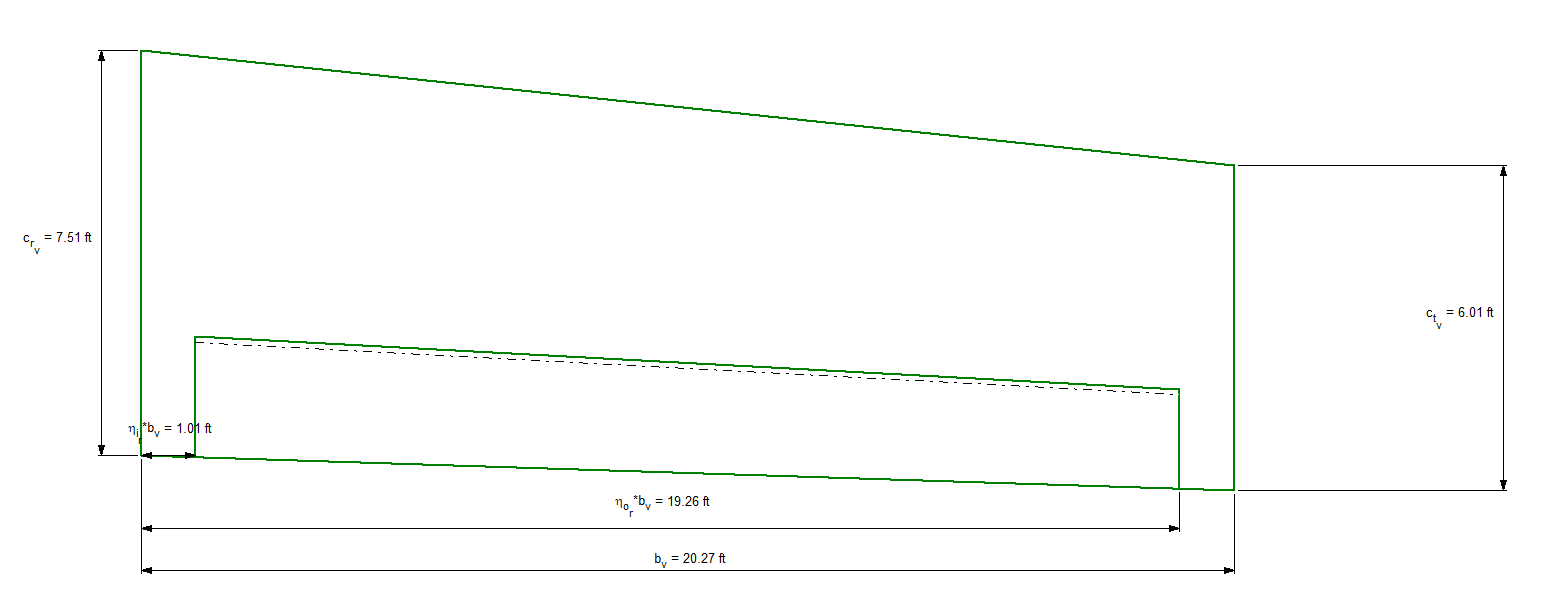
\includegraphics[width=\textwidth]{Report3Printouts/Empannage/Vertical_rudder_plot.png}
    \caption{Rudder control surface layout}
    \label{fig:vertical_rudder_plot}
\end{figure}


\subsection{AAA: Stability Derivatives}

\begin{figure}[H]
    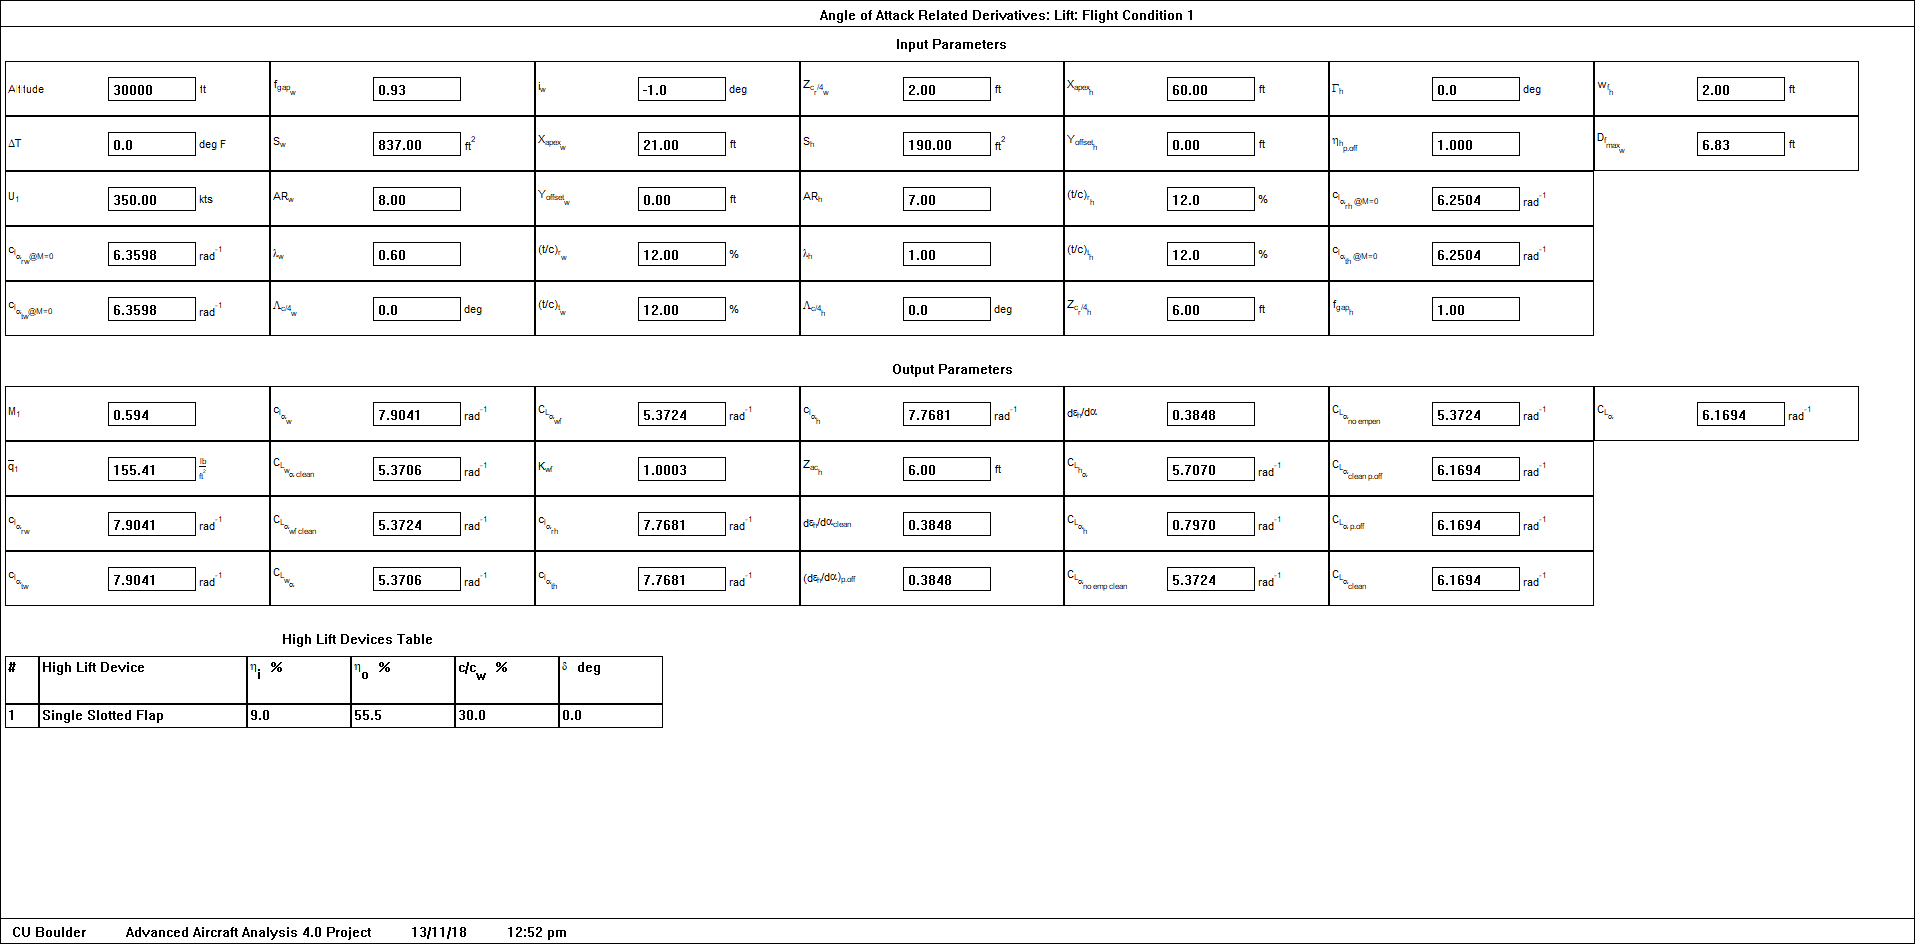
\includegraphics[width=\textwidth]{Report3Printouts/Stability/CL_alpha.png}
    \caption{Calculations of derivatives of $C_L$}
    \label{fig:cl_alpha}
\end{figure}

\begin{figure}[H]
    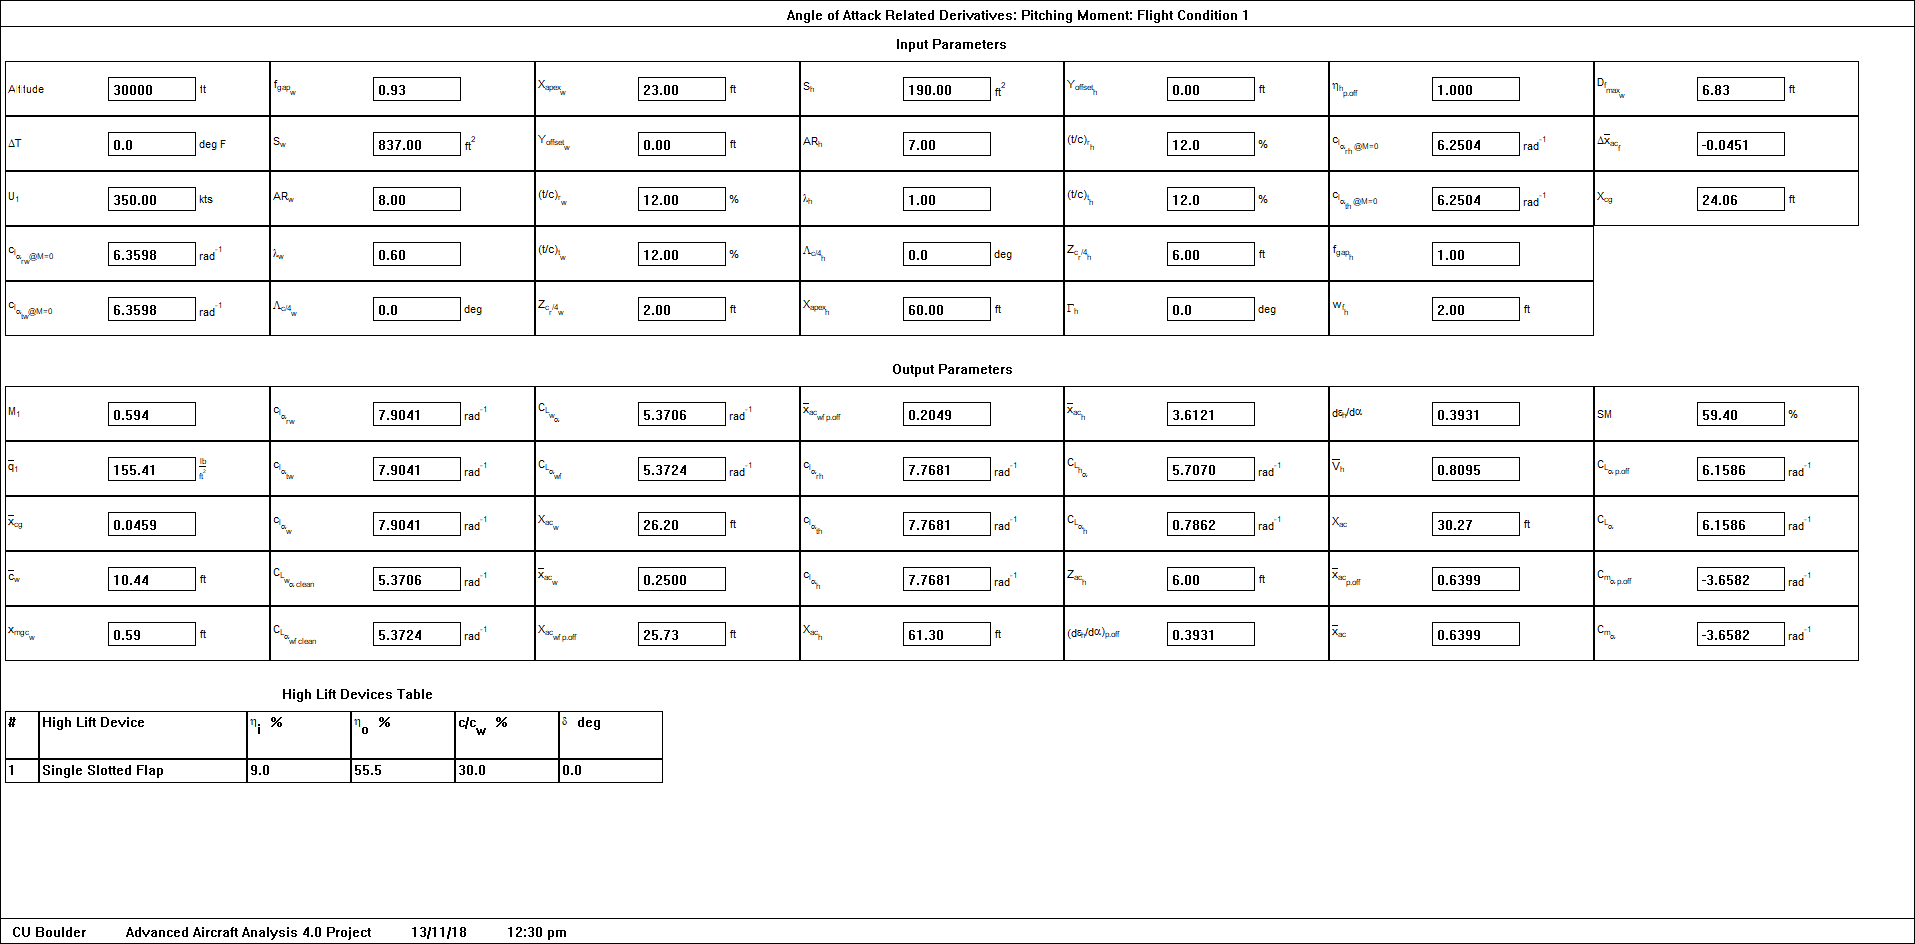
\includegraphics[width=\textwidth]{Report3Printouts/Stability/CM_alpha.png}
    \caption{Initial static margin calculation}
    \label{fig:cm_alpha}
\end{figure}

\begin{figure}[H]
    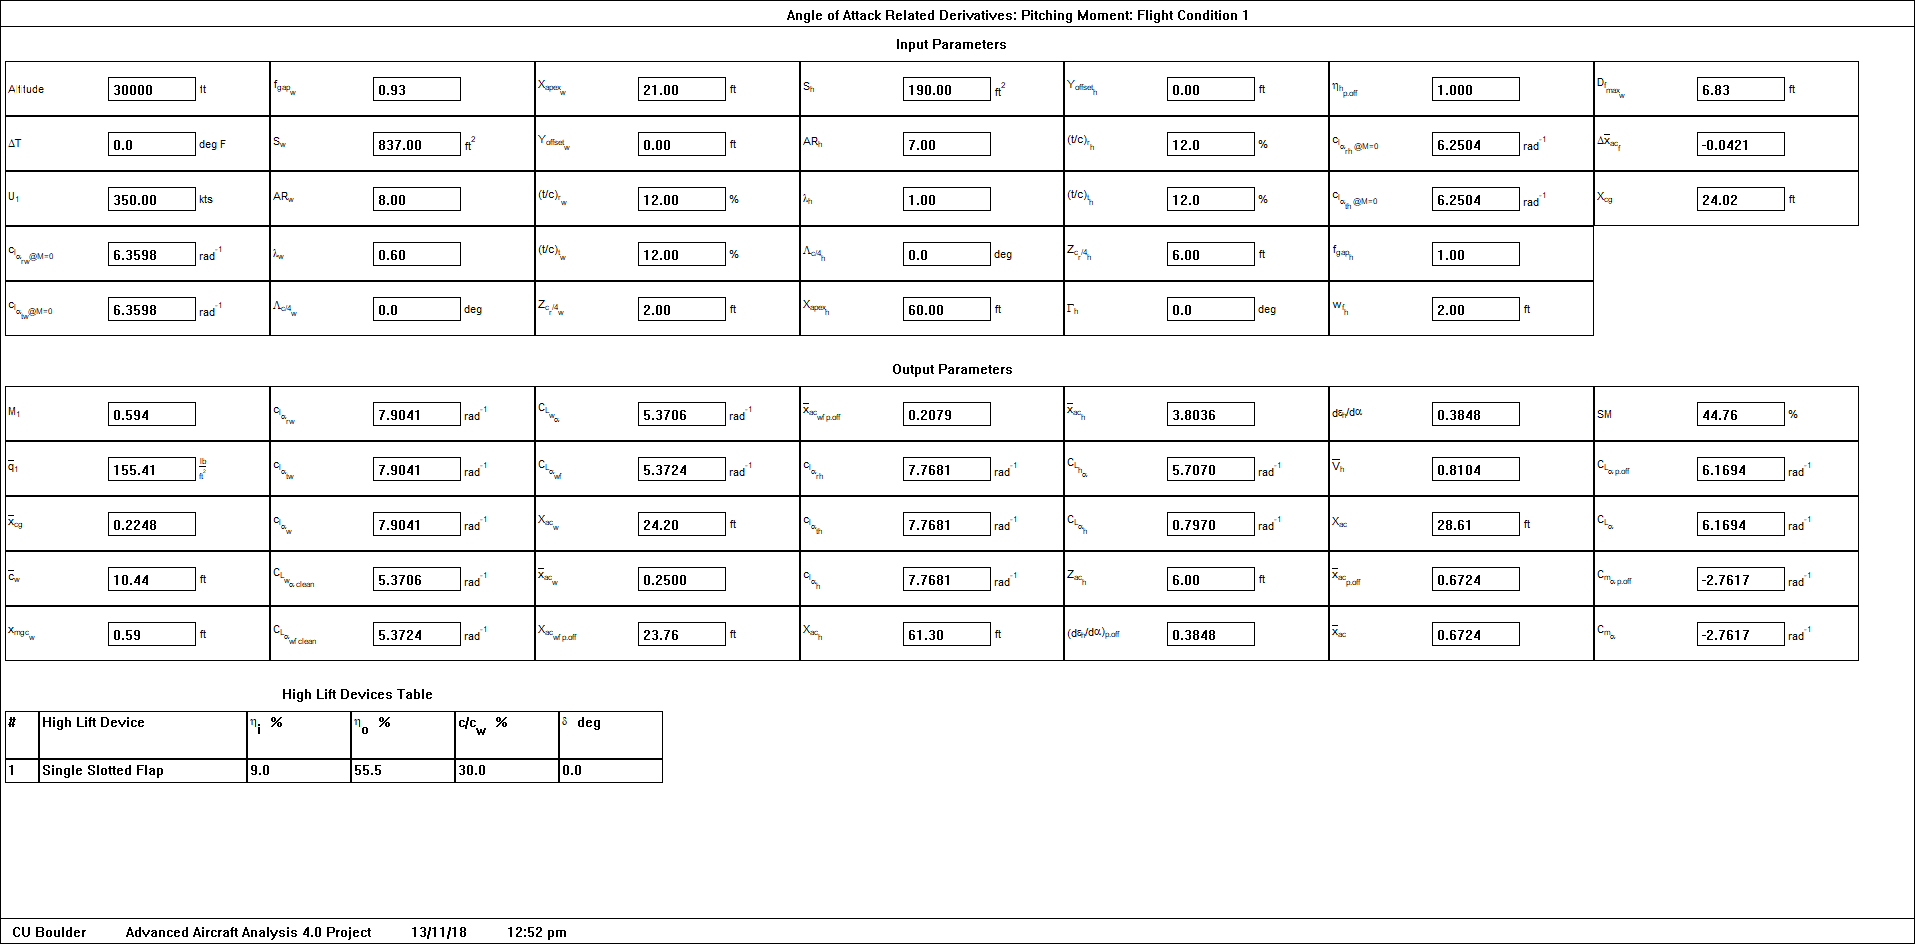
\includegraphics[width=\textwidth]{Report3Printouts/Stability/CM_alpha_final.png}
    \caption{Revised static margin calculation}
    \label{fig:cm_alpha_final}
\end{figure}

\begin{figure}[H]
    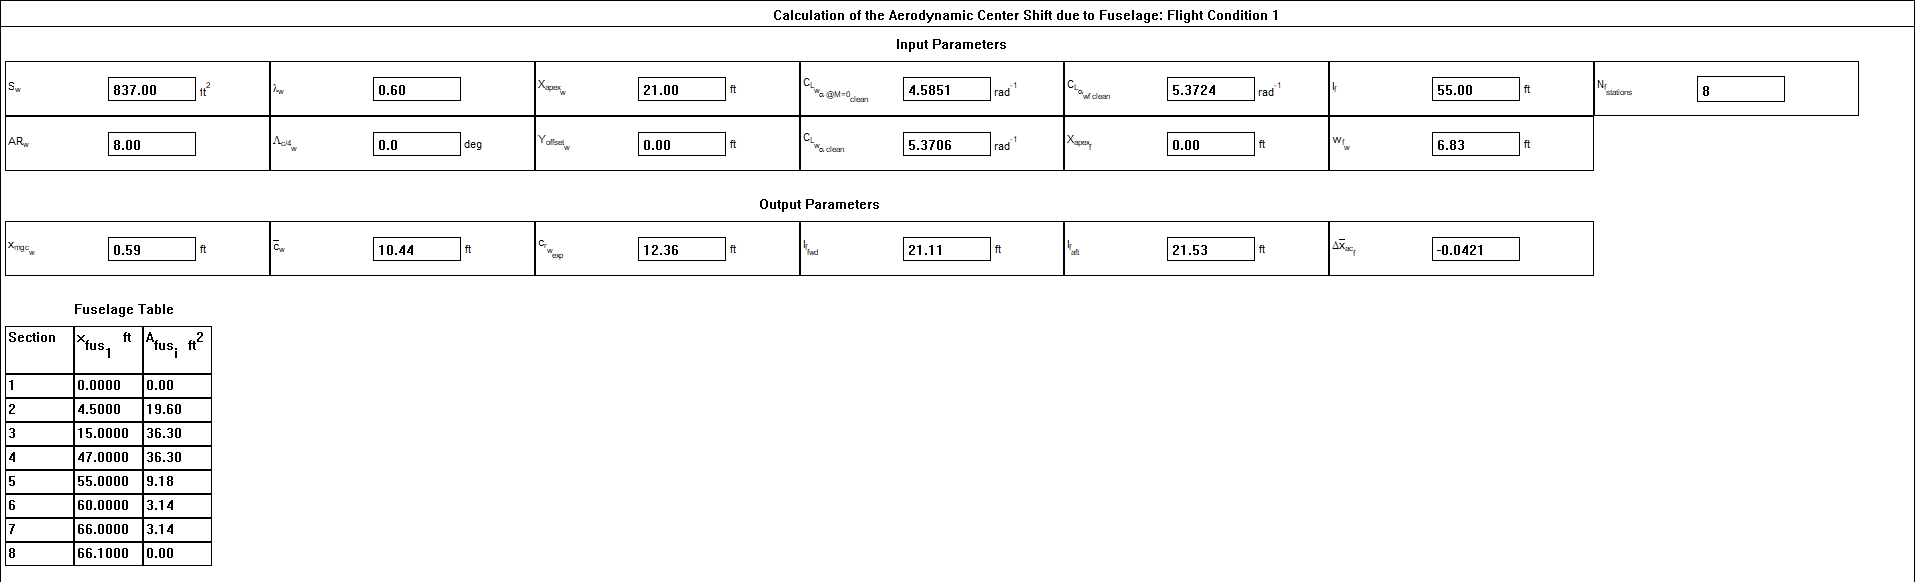
\includegraphics[width=\textwidth]{Report3Printouts/Stability/delta_x_ac_f_cropped.png}
    \caption{Change in aerodynamic center due to fuselage influence}
    \label{fig:delta_x_ac_f}
\end{figure}

\end{document}

